\chapter{Módulo 6: Fuente de poder externa}

\section{Paso 1:}

Instalar regulador U4. LM7805. Es recomendable doblar las patitas antes de posicionarlo y soldarlo

\begin{figure}[h]
	\centering
	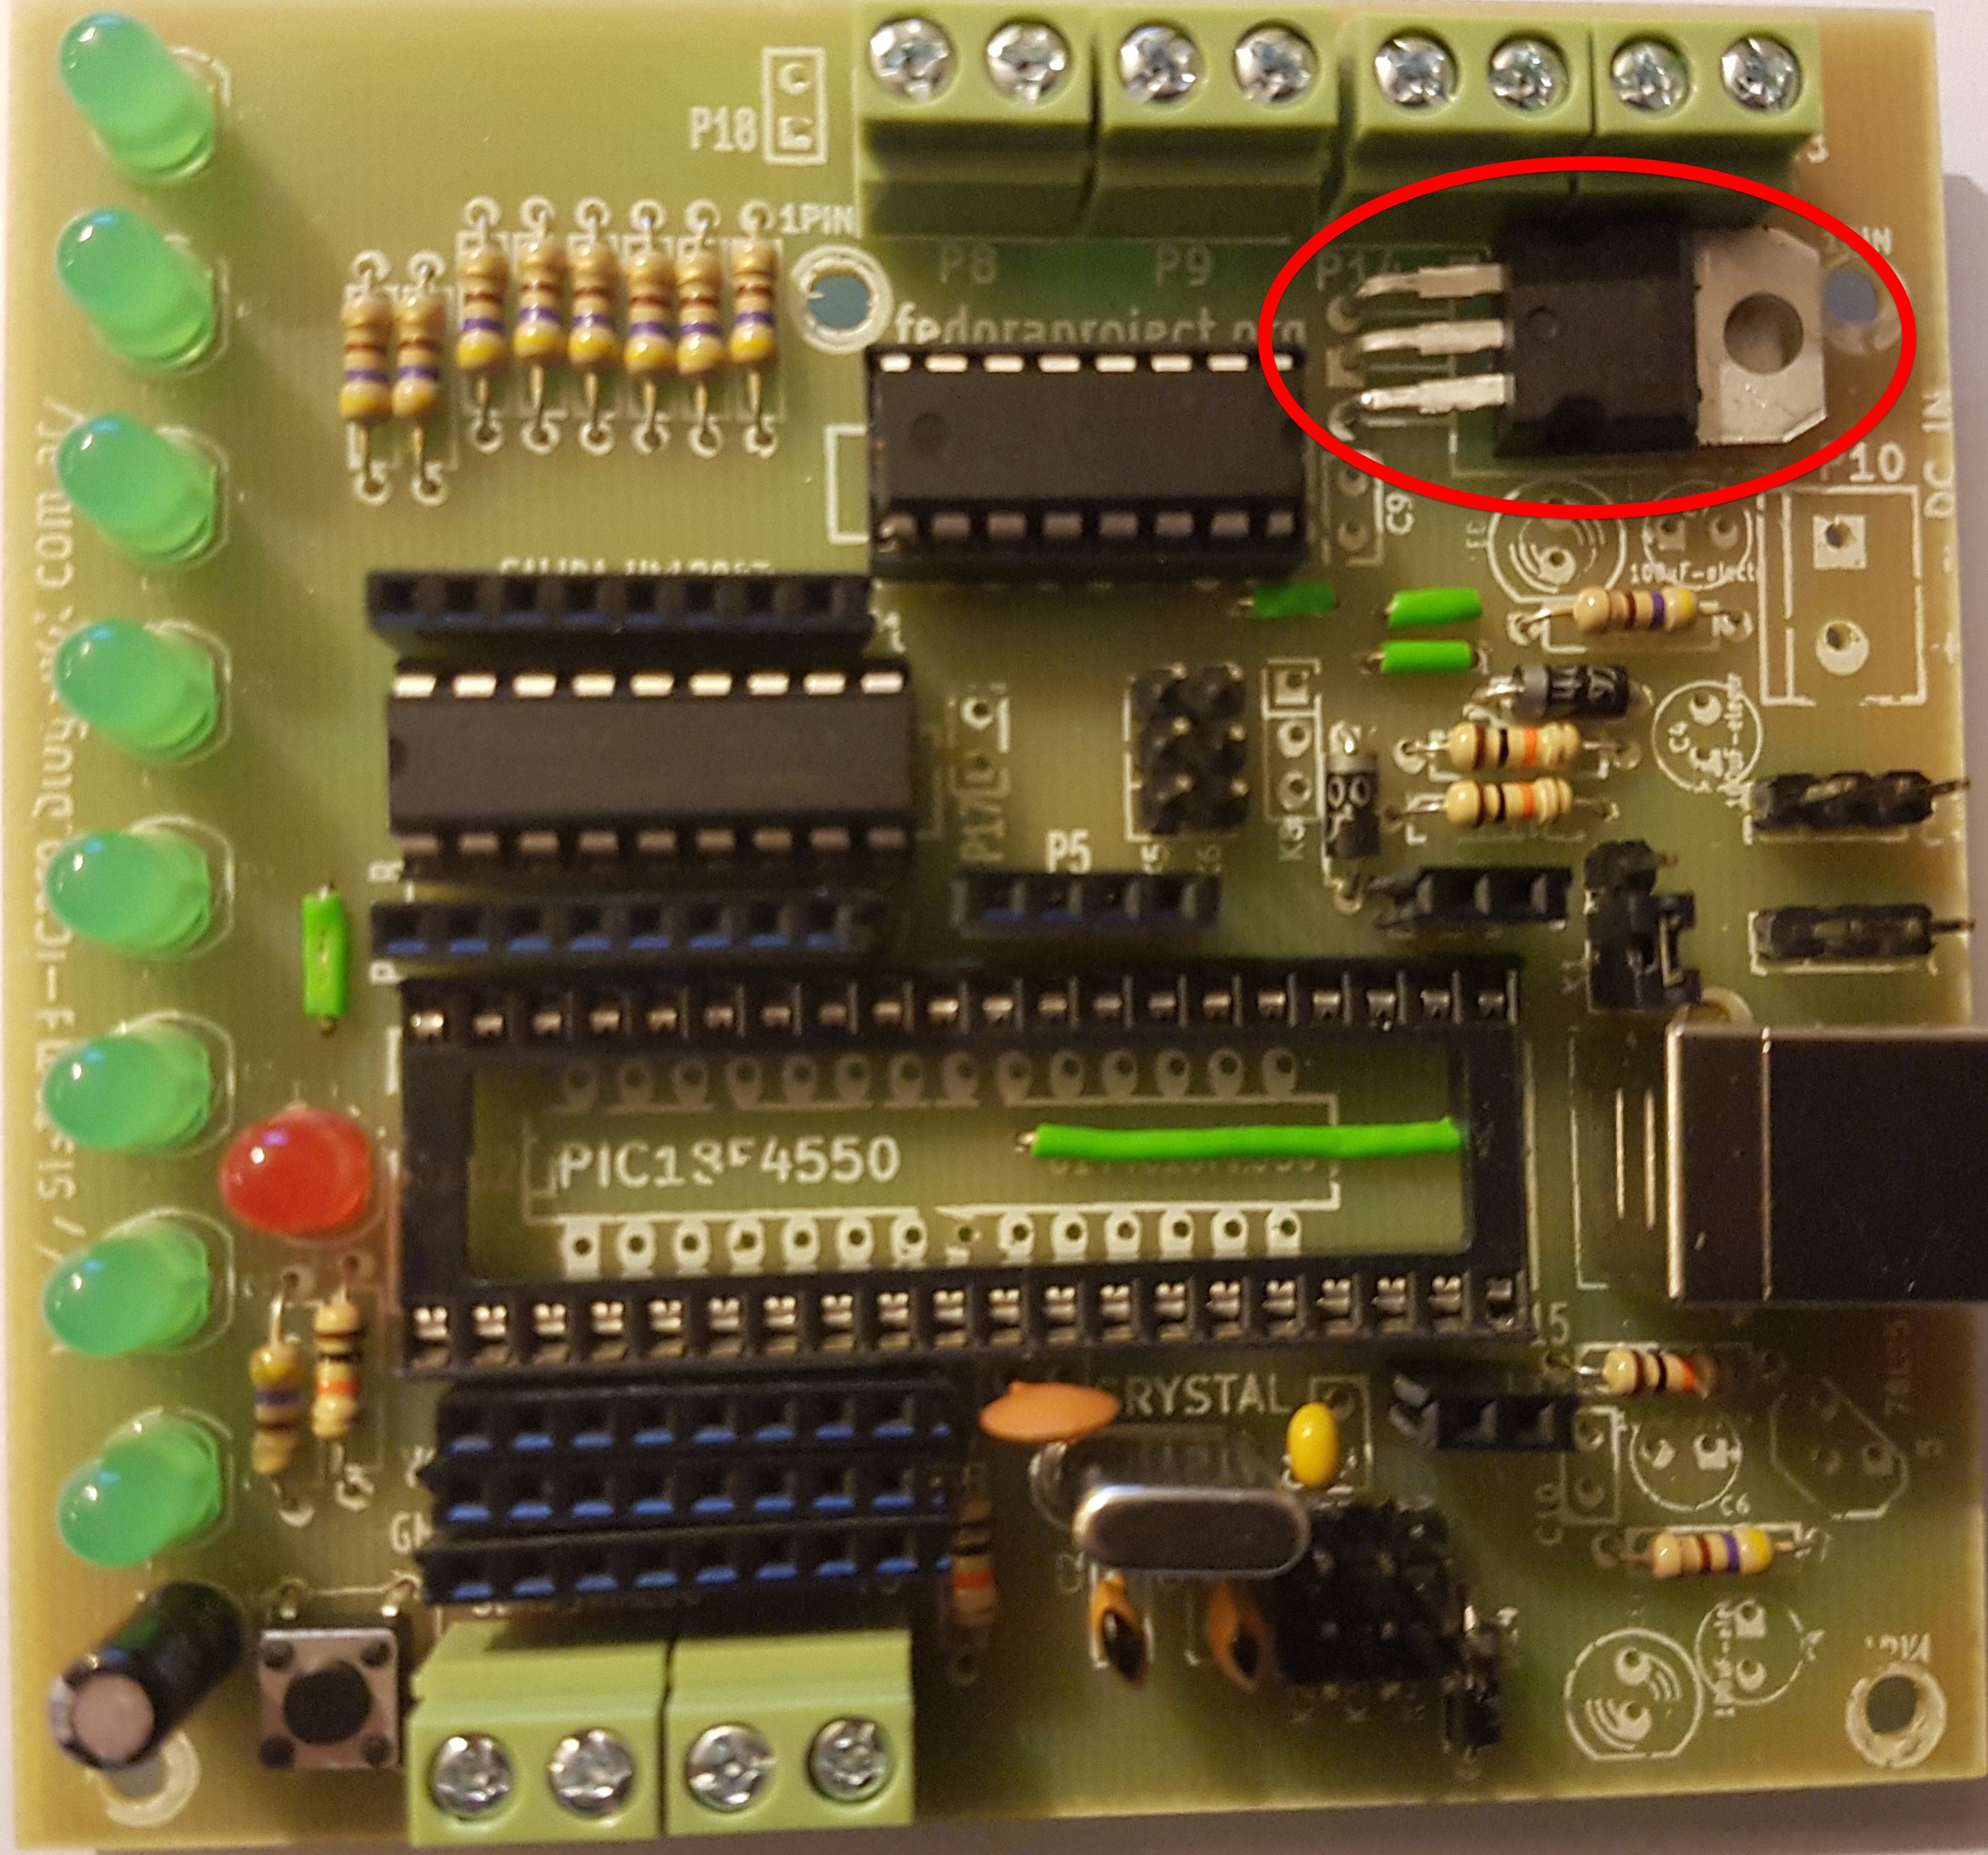
\includegraphics[width=0.8\linewidth]{Modulo_6/M6_1}
	\caption{Módulo 6 - Paso 1}
	\label{fig:M6_1}
\end{figure}

\newpage

\section{Paso 2:}

Instalar capacitor cerámico 0.1uF C9

\begin{figure}[h]
	\centering
	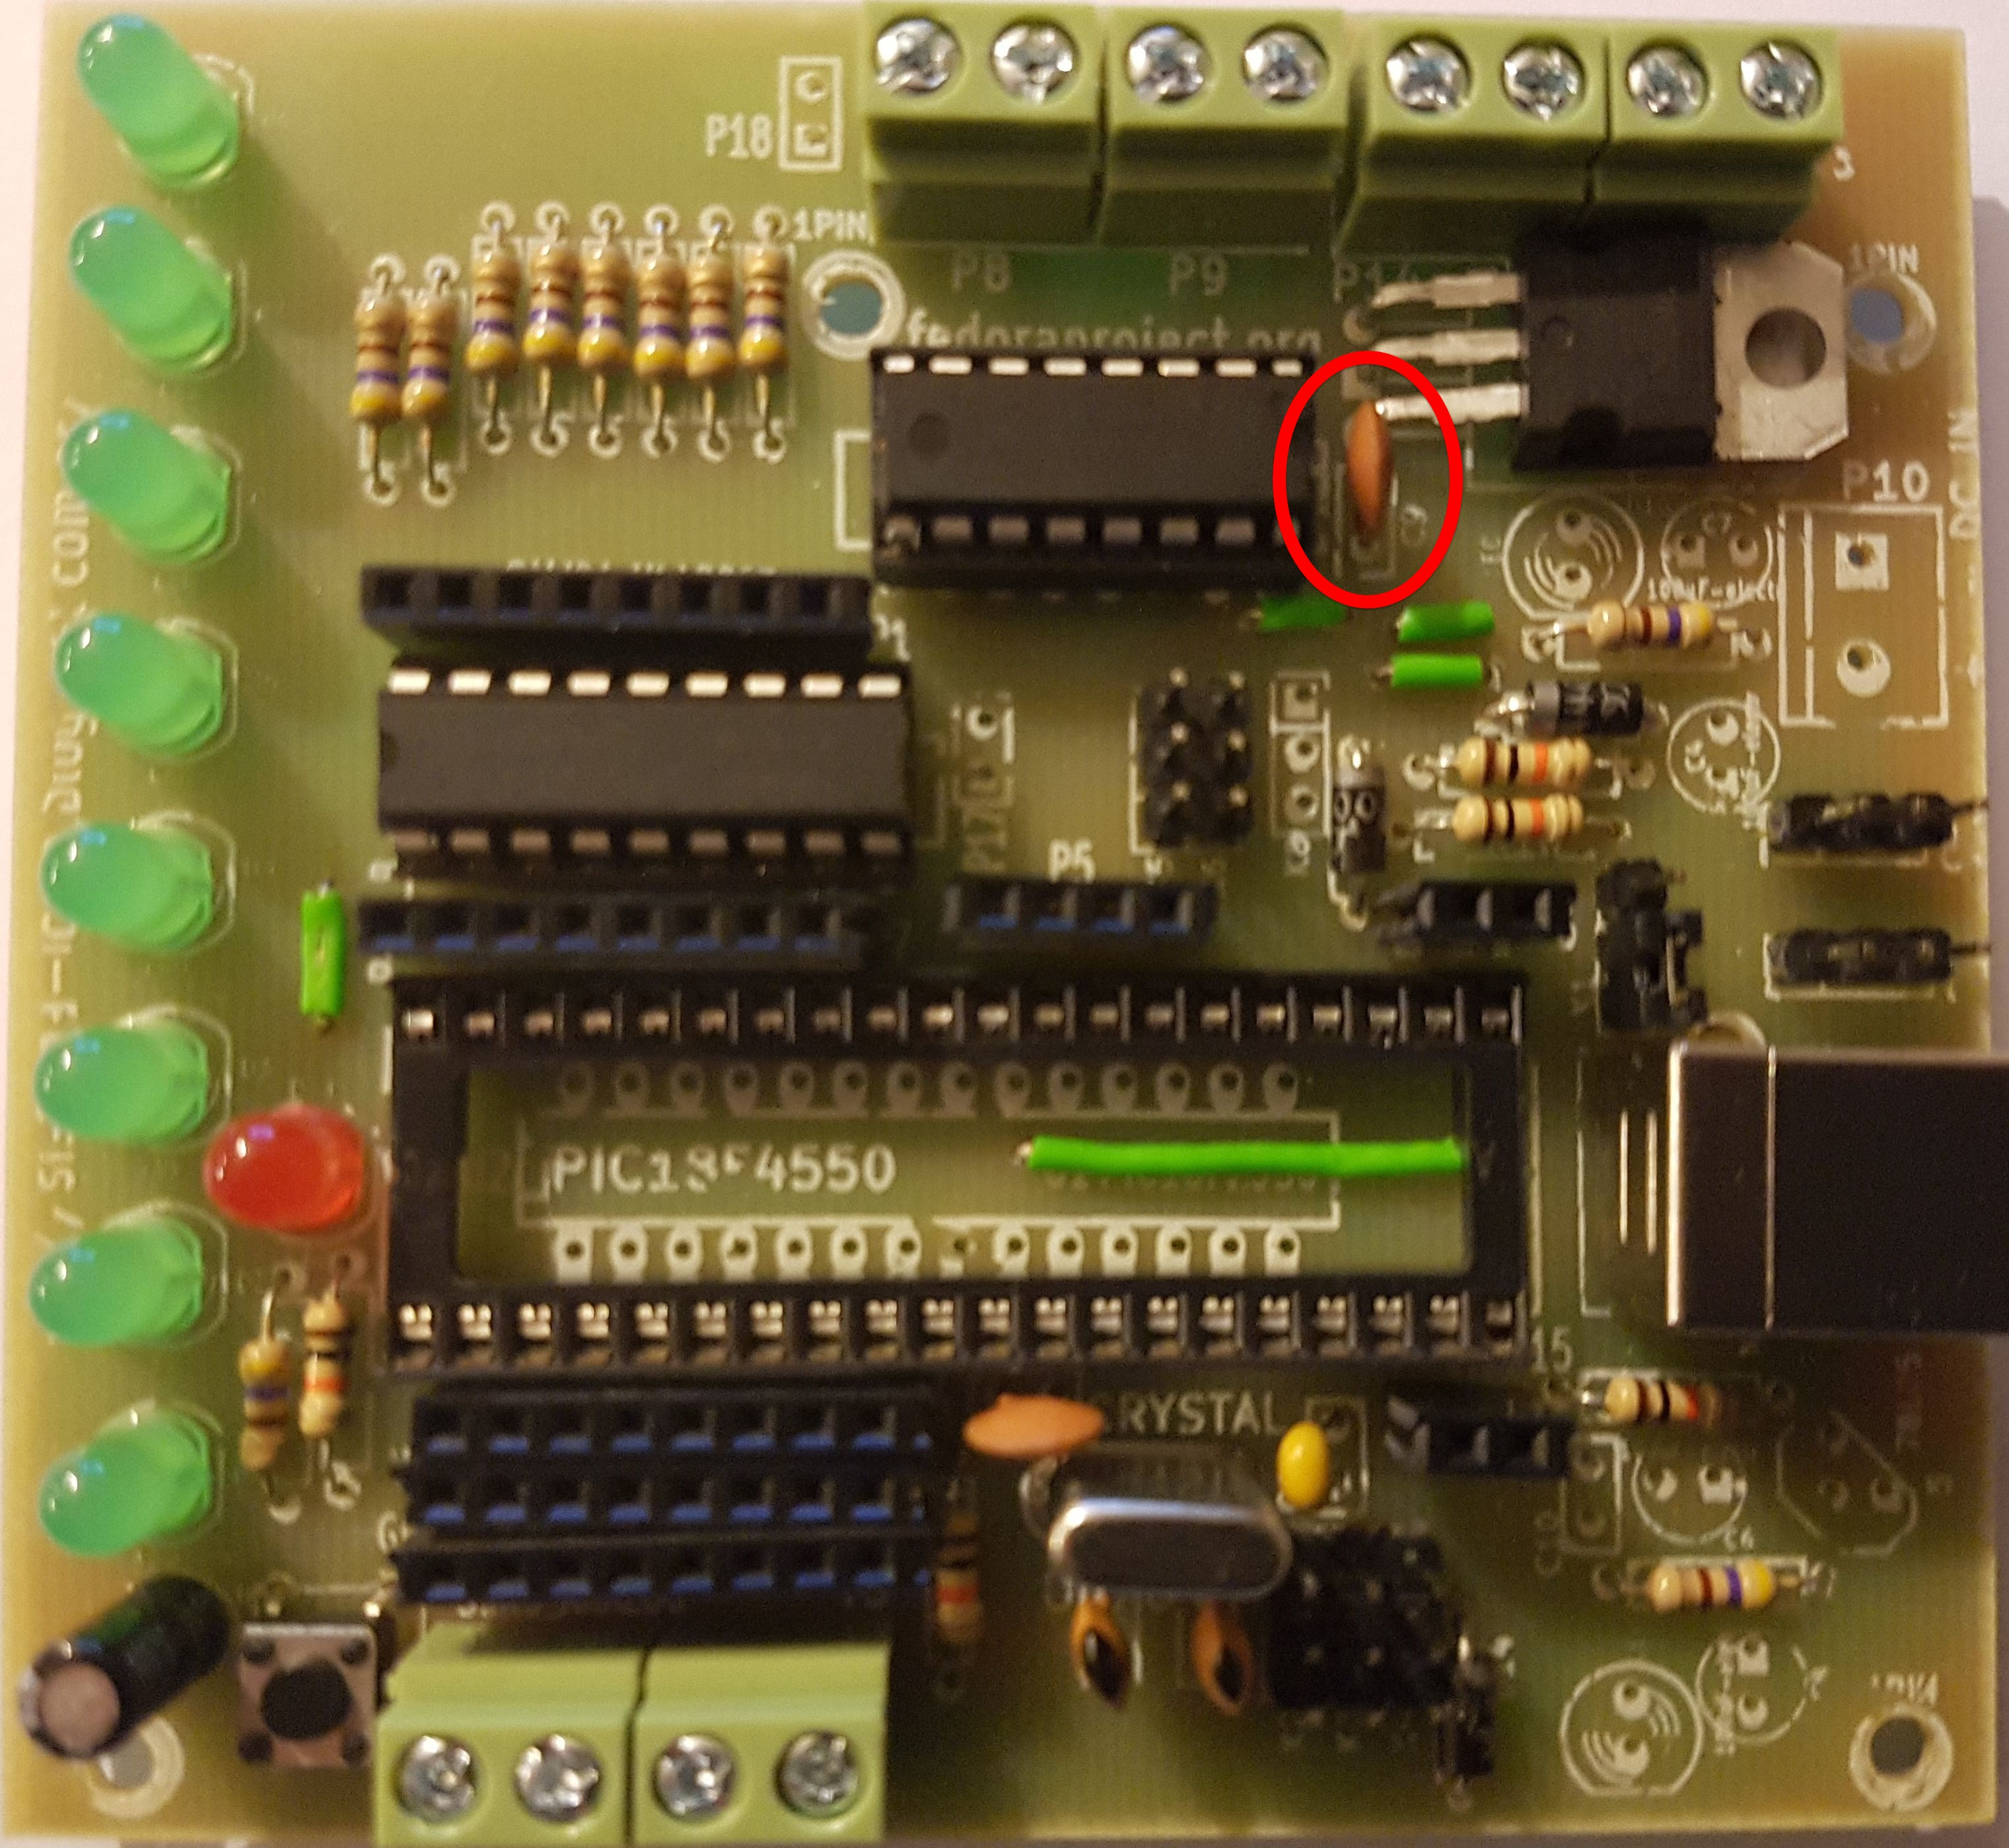
\includegraphics[width=0.8\linewidth]{Modulo_6/M6_2}
	\caption{Módulo 6 - Paso 2}
	\label{fig:M6_2}
\end{figure}

\newpage

\section{Paso 3:}

Instalar led de alimentación de motores. D10 (Se recomienda amarillo)

\begin{figure}[h]
	\centering
	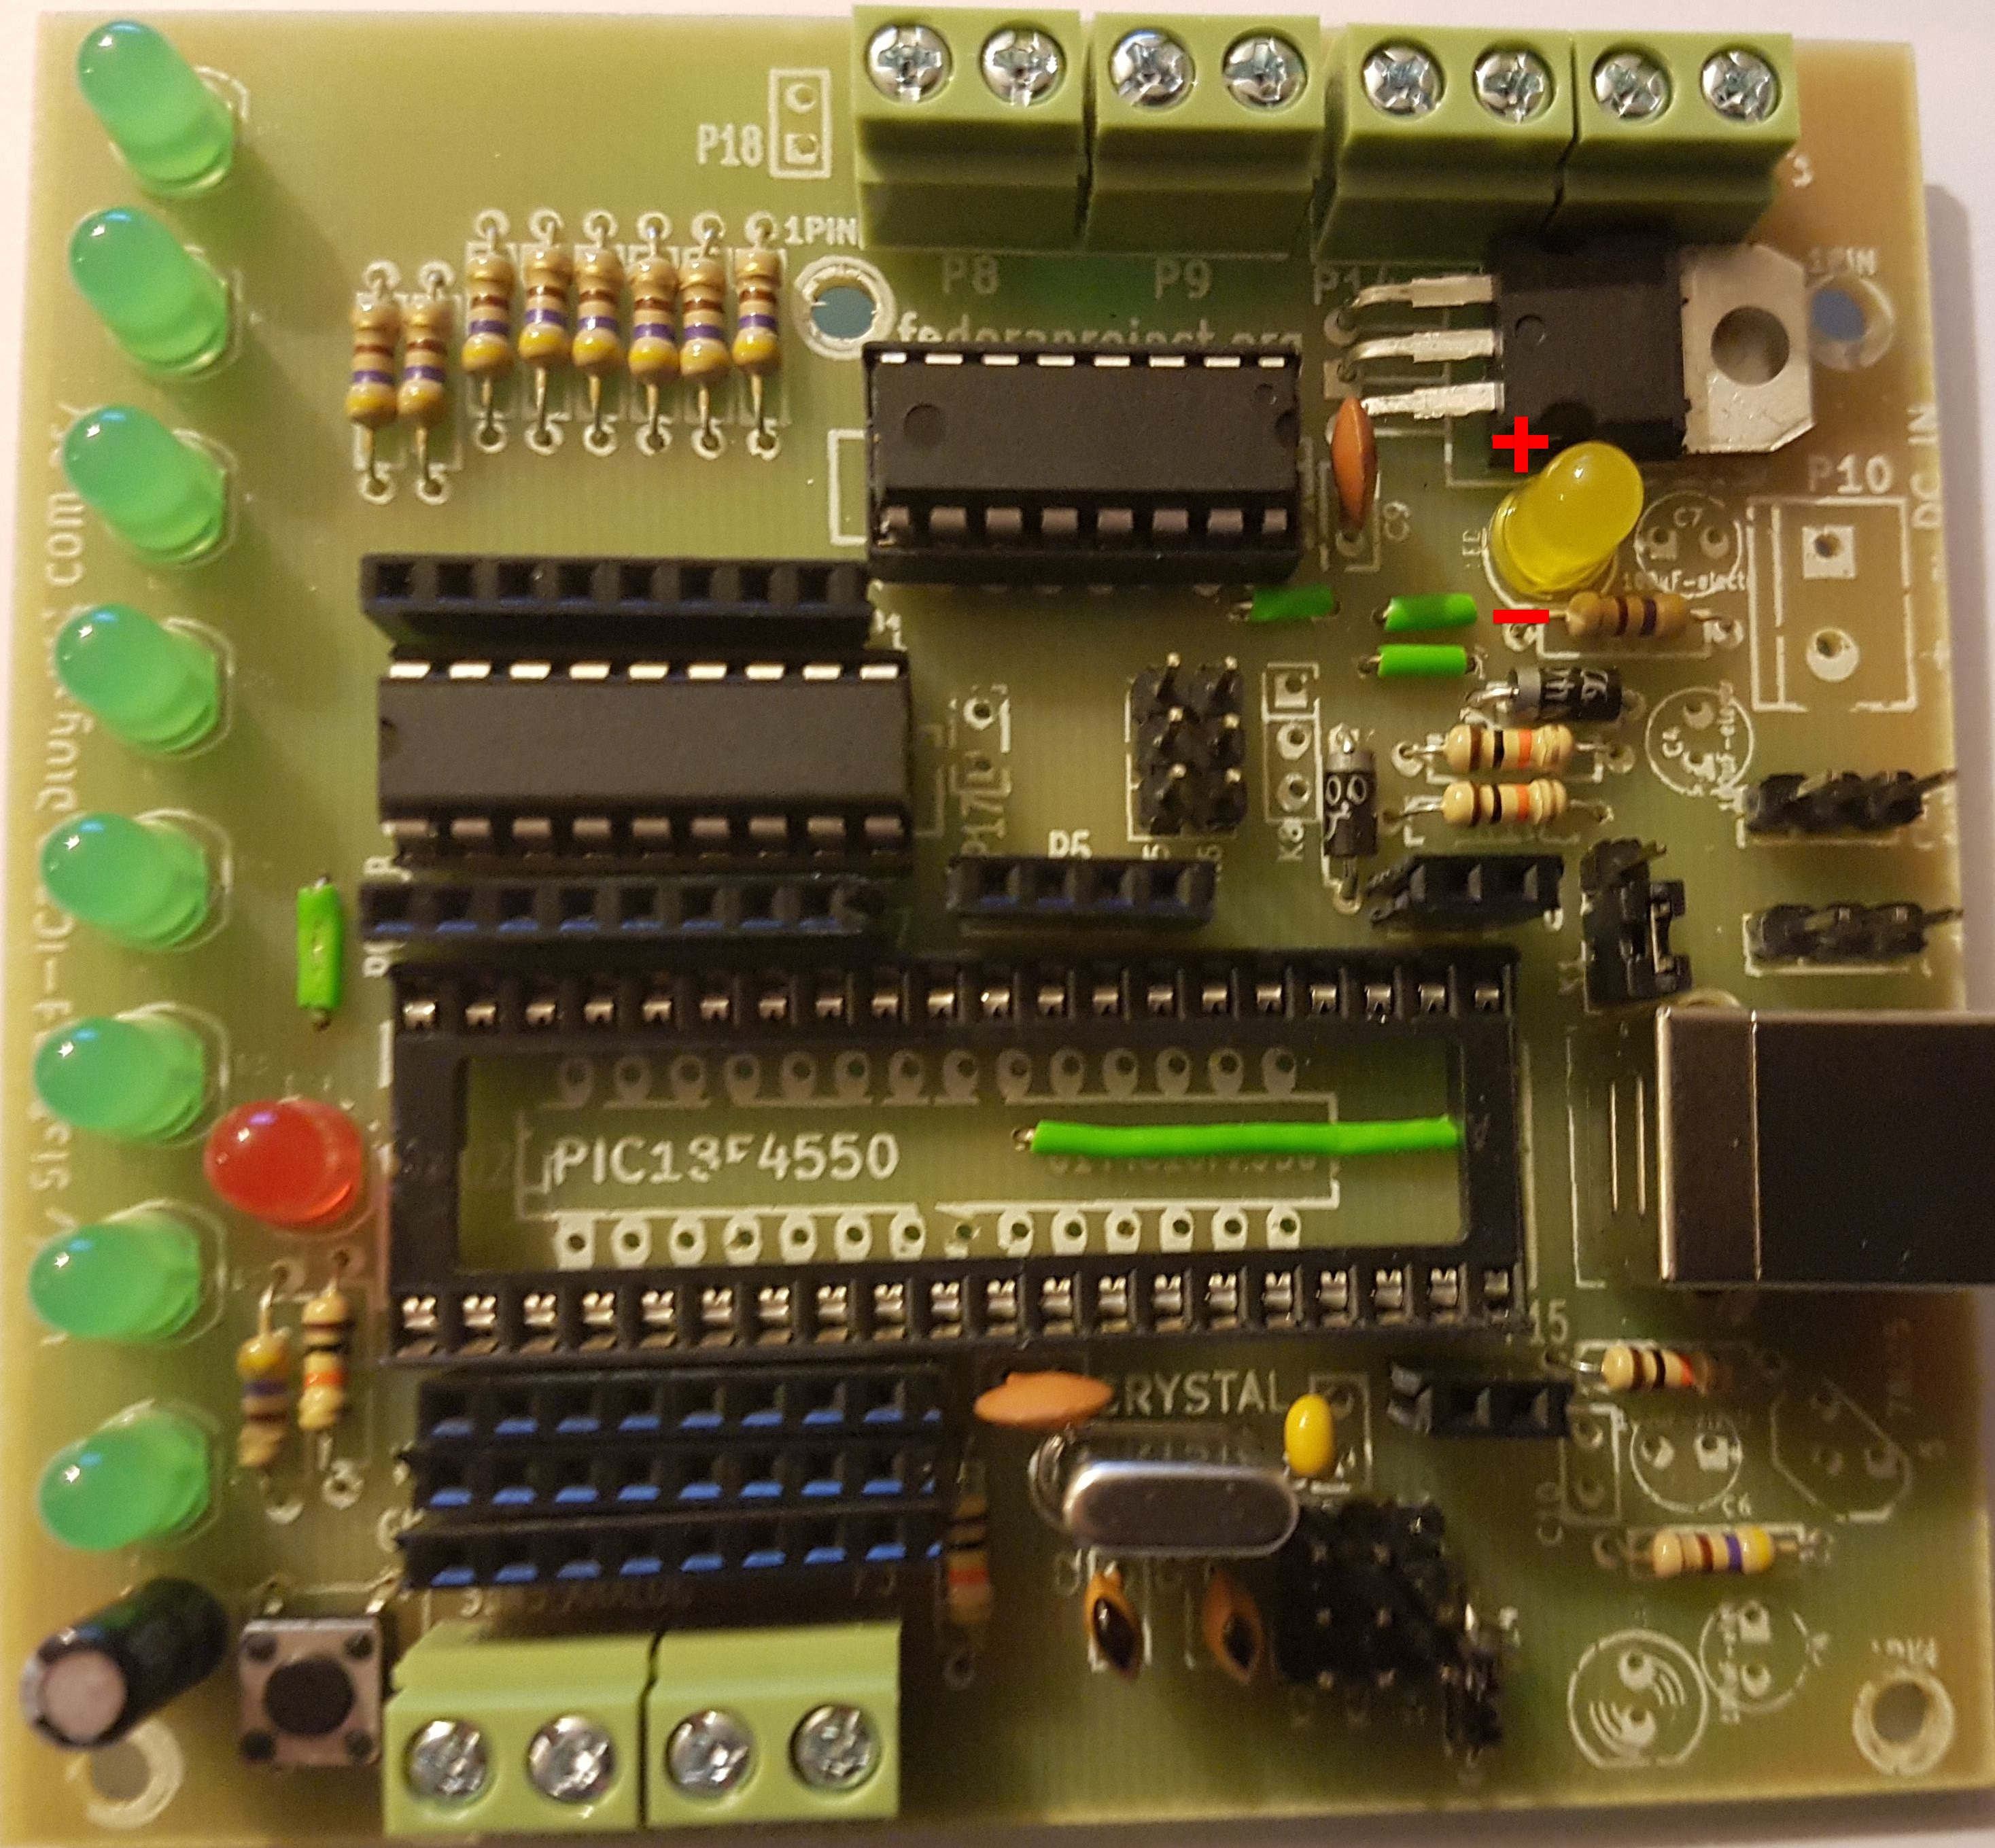
\includegraphics[width=0.8\linewidth]{Modulo_6/M6_3}
	\caption{Módulo 6 - Paso 3}
	\label{fig:M6_3}
\end{figure}

\newpage

\section{Paso 4:}

Instalar capacitores electrolíticos 100uF C4 y C7

\begin{figure}[h]
	\centering
	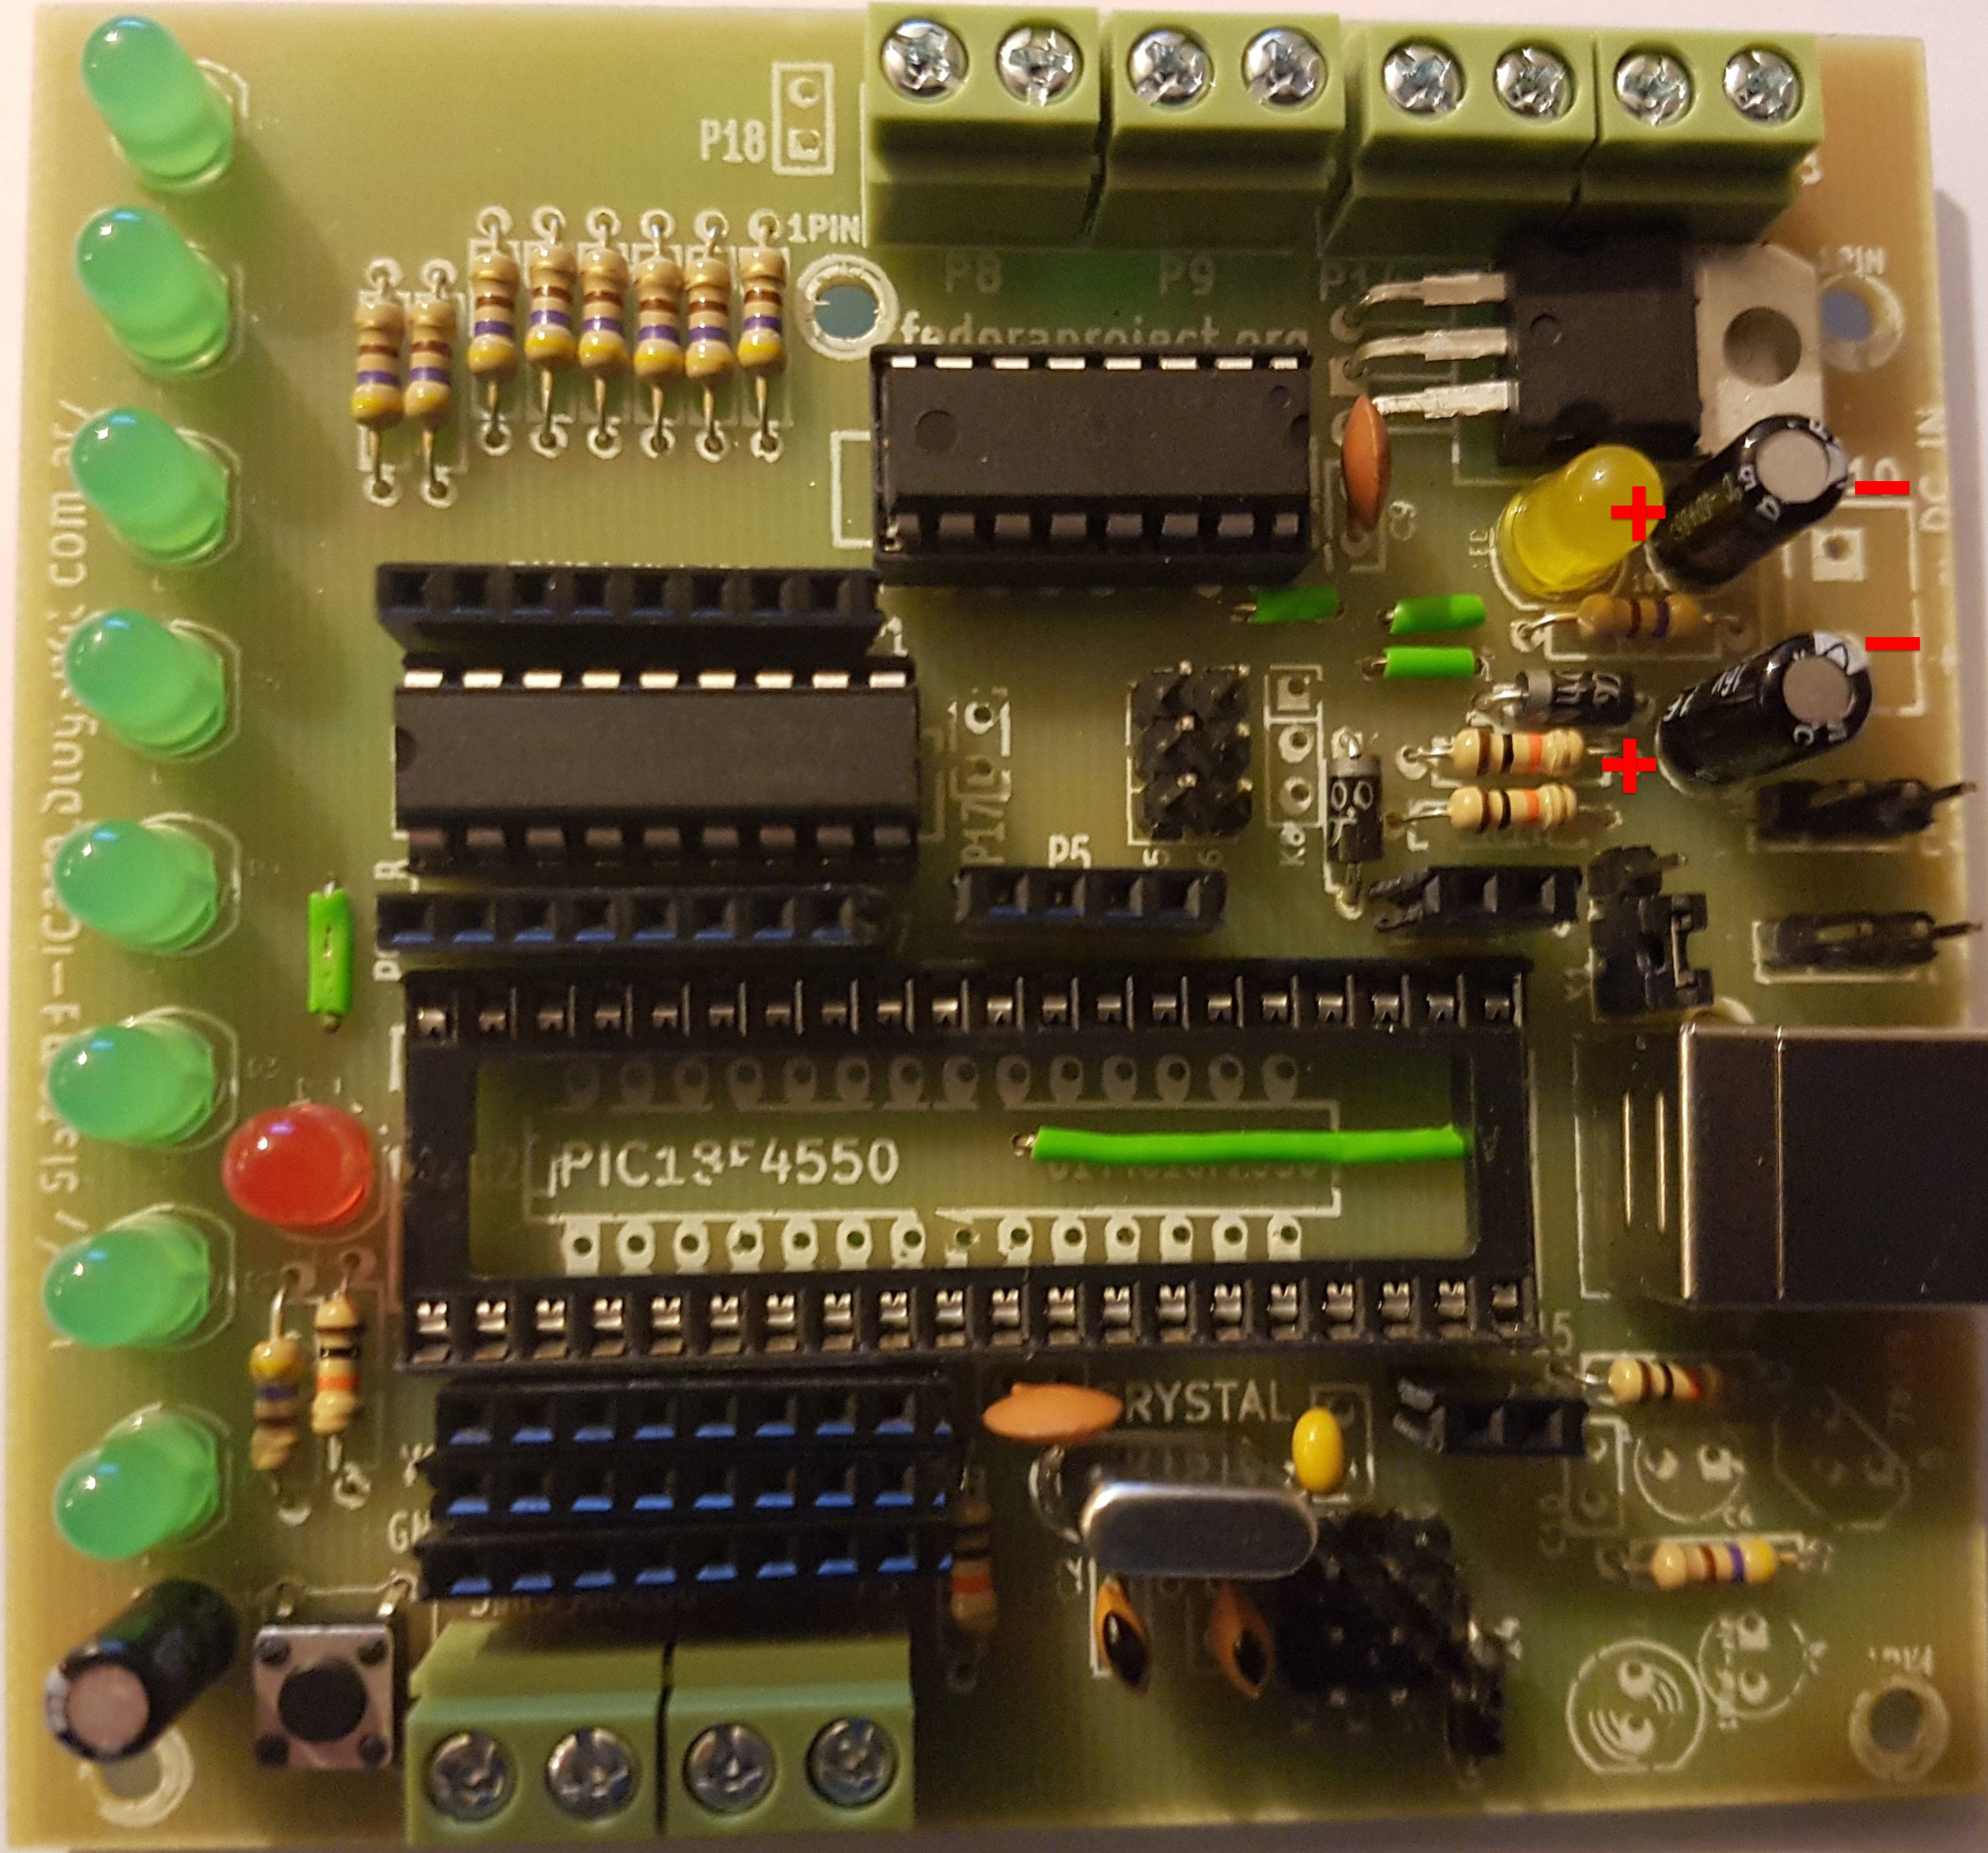
\includegraphics[width=0.8\linewidth]{Modulo_6/M6_4}
	\caption{Módulo 6 - Paso 4}
	\label{fig:M6_4}
\end{figure}

\newpage

\section{Paso 5:}

Instalar bornera de dos posiciones para alimentación externa. P10

\begin{figure}[h]
	\centering
	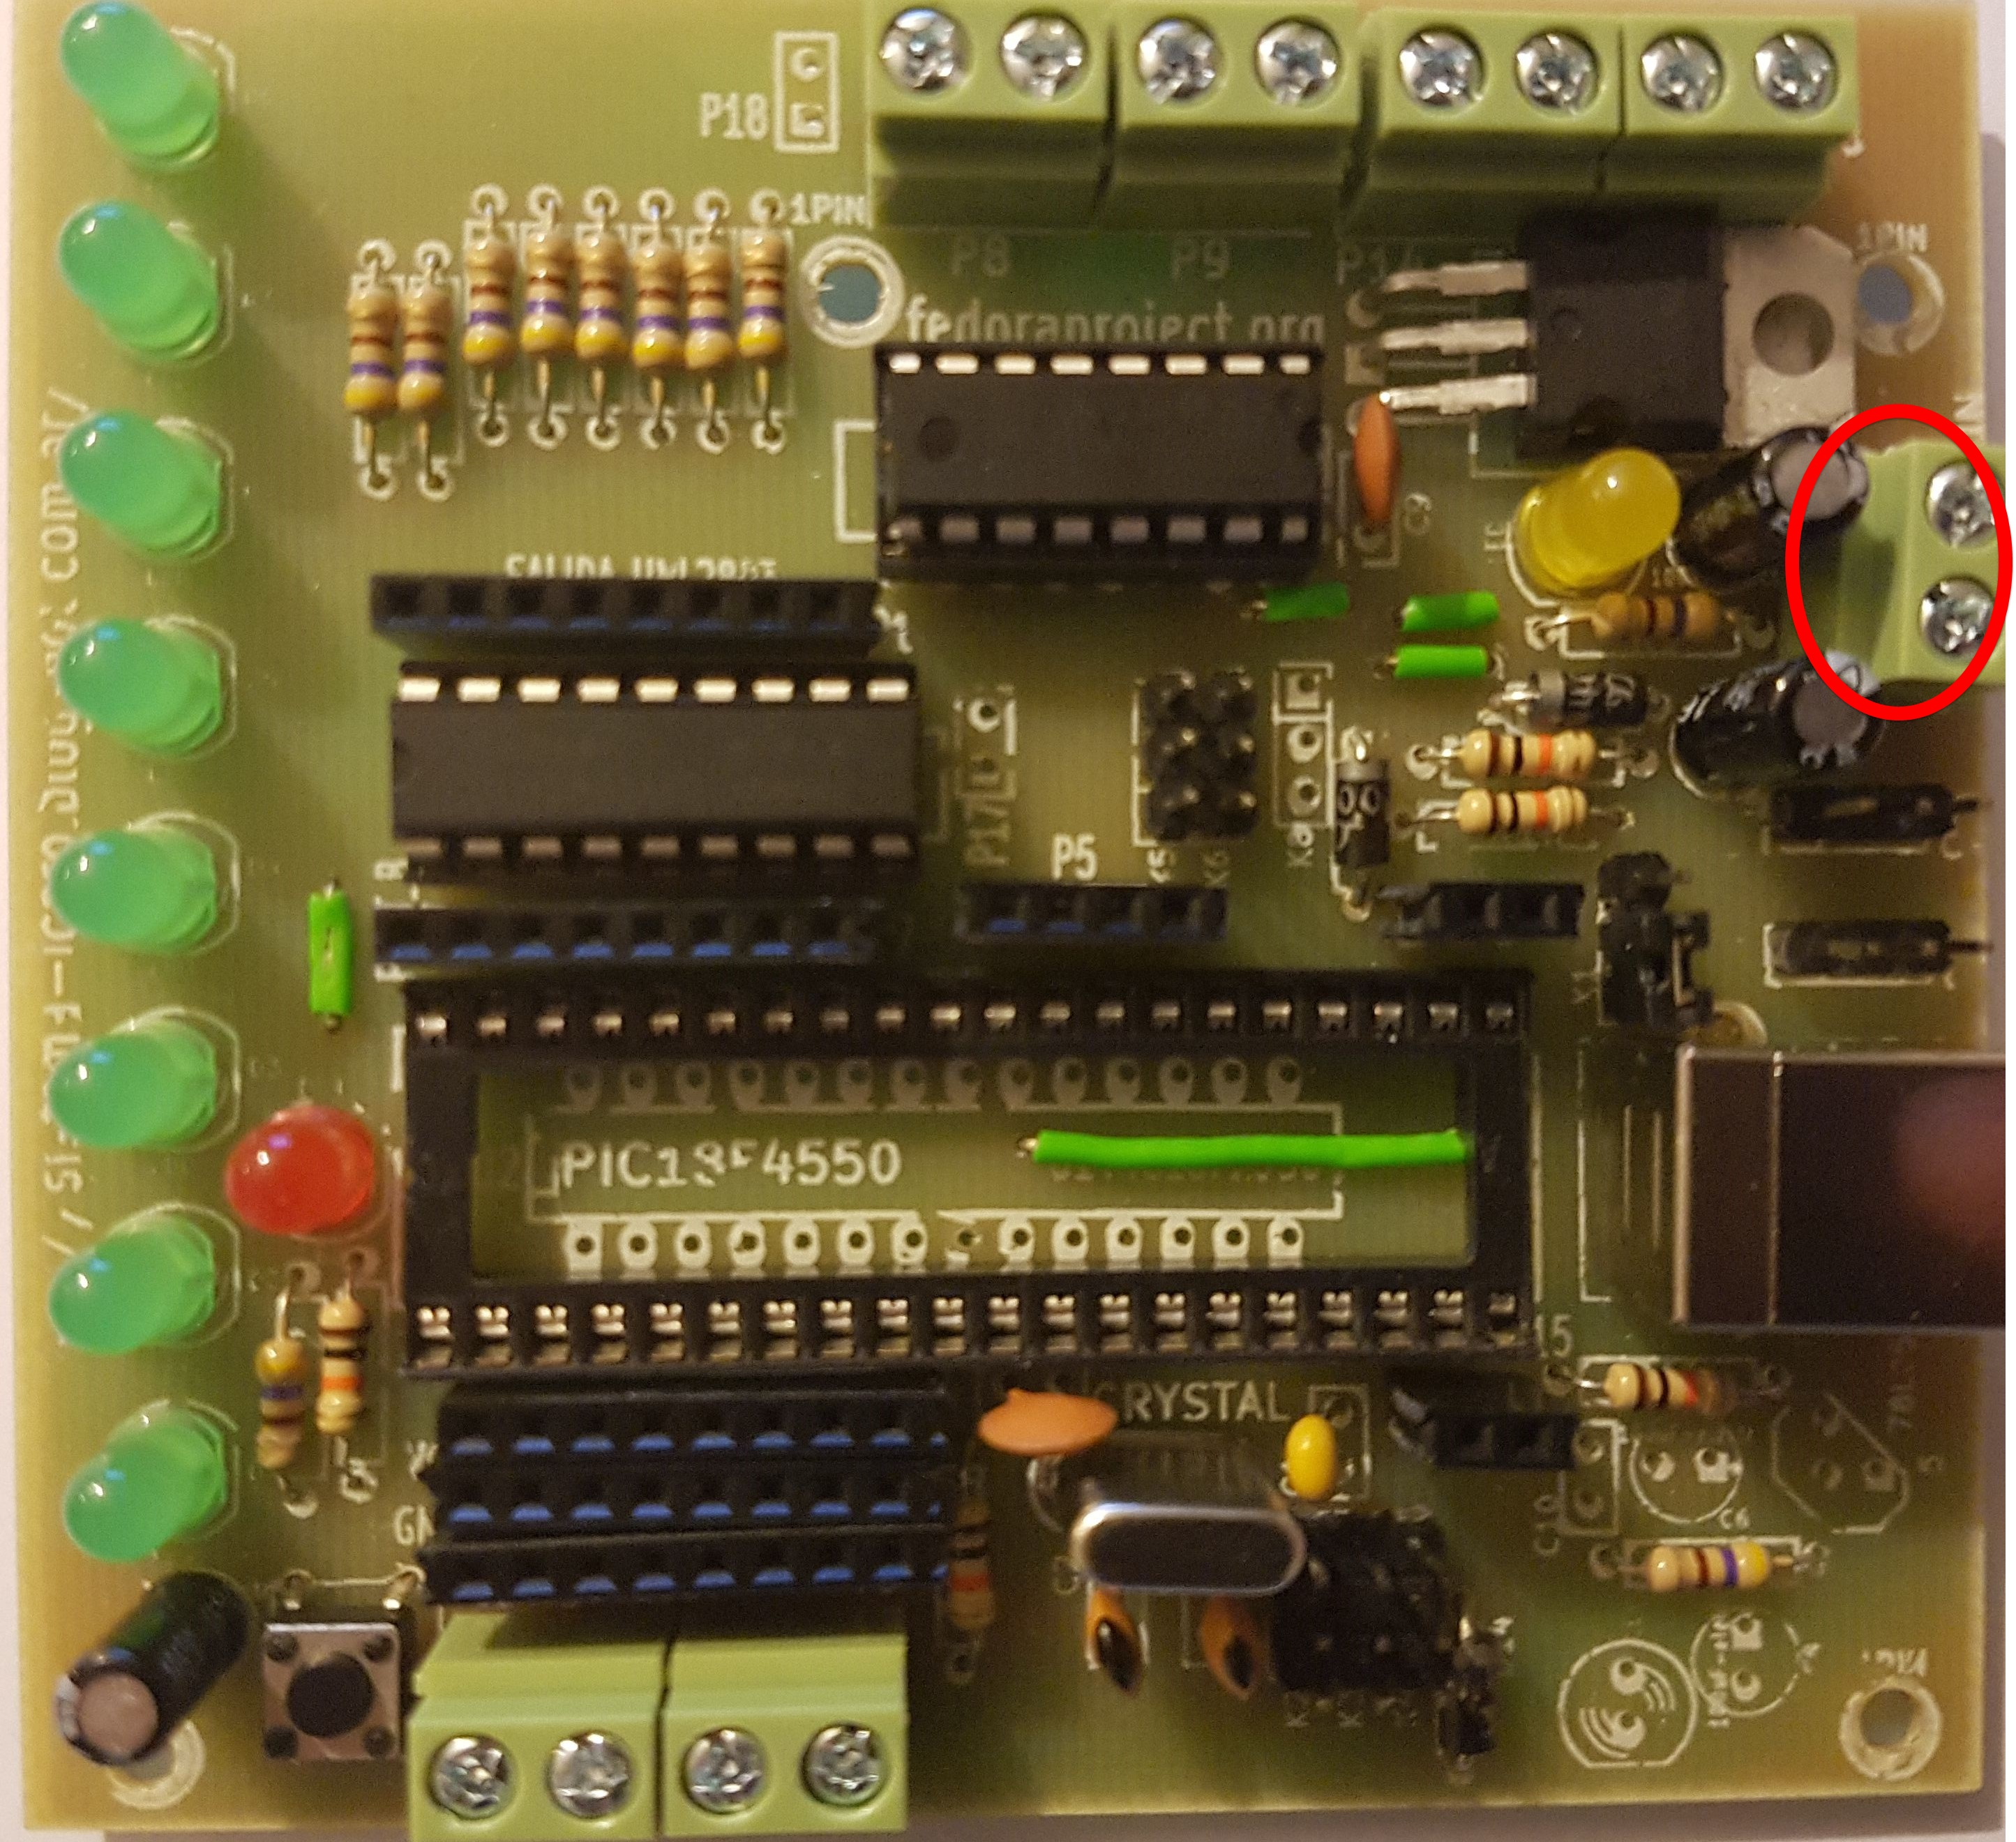
\includegraphics[width=0.8\linewidth]{Modulo_6/M6_5}
	\caption{Módulo 6 - Paso 5}
	\label{fig:M6_5}
\end{figure}

\newpage

\section{Paso 6:}

Instalar capacitor cerámico 0.1uF C10

\begin{figure}[h]
	\centering
	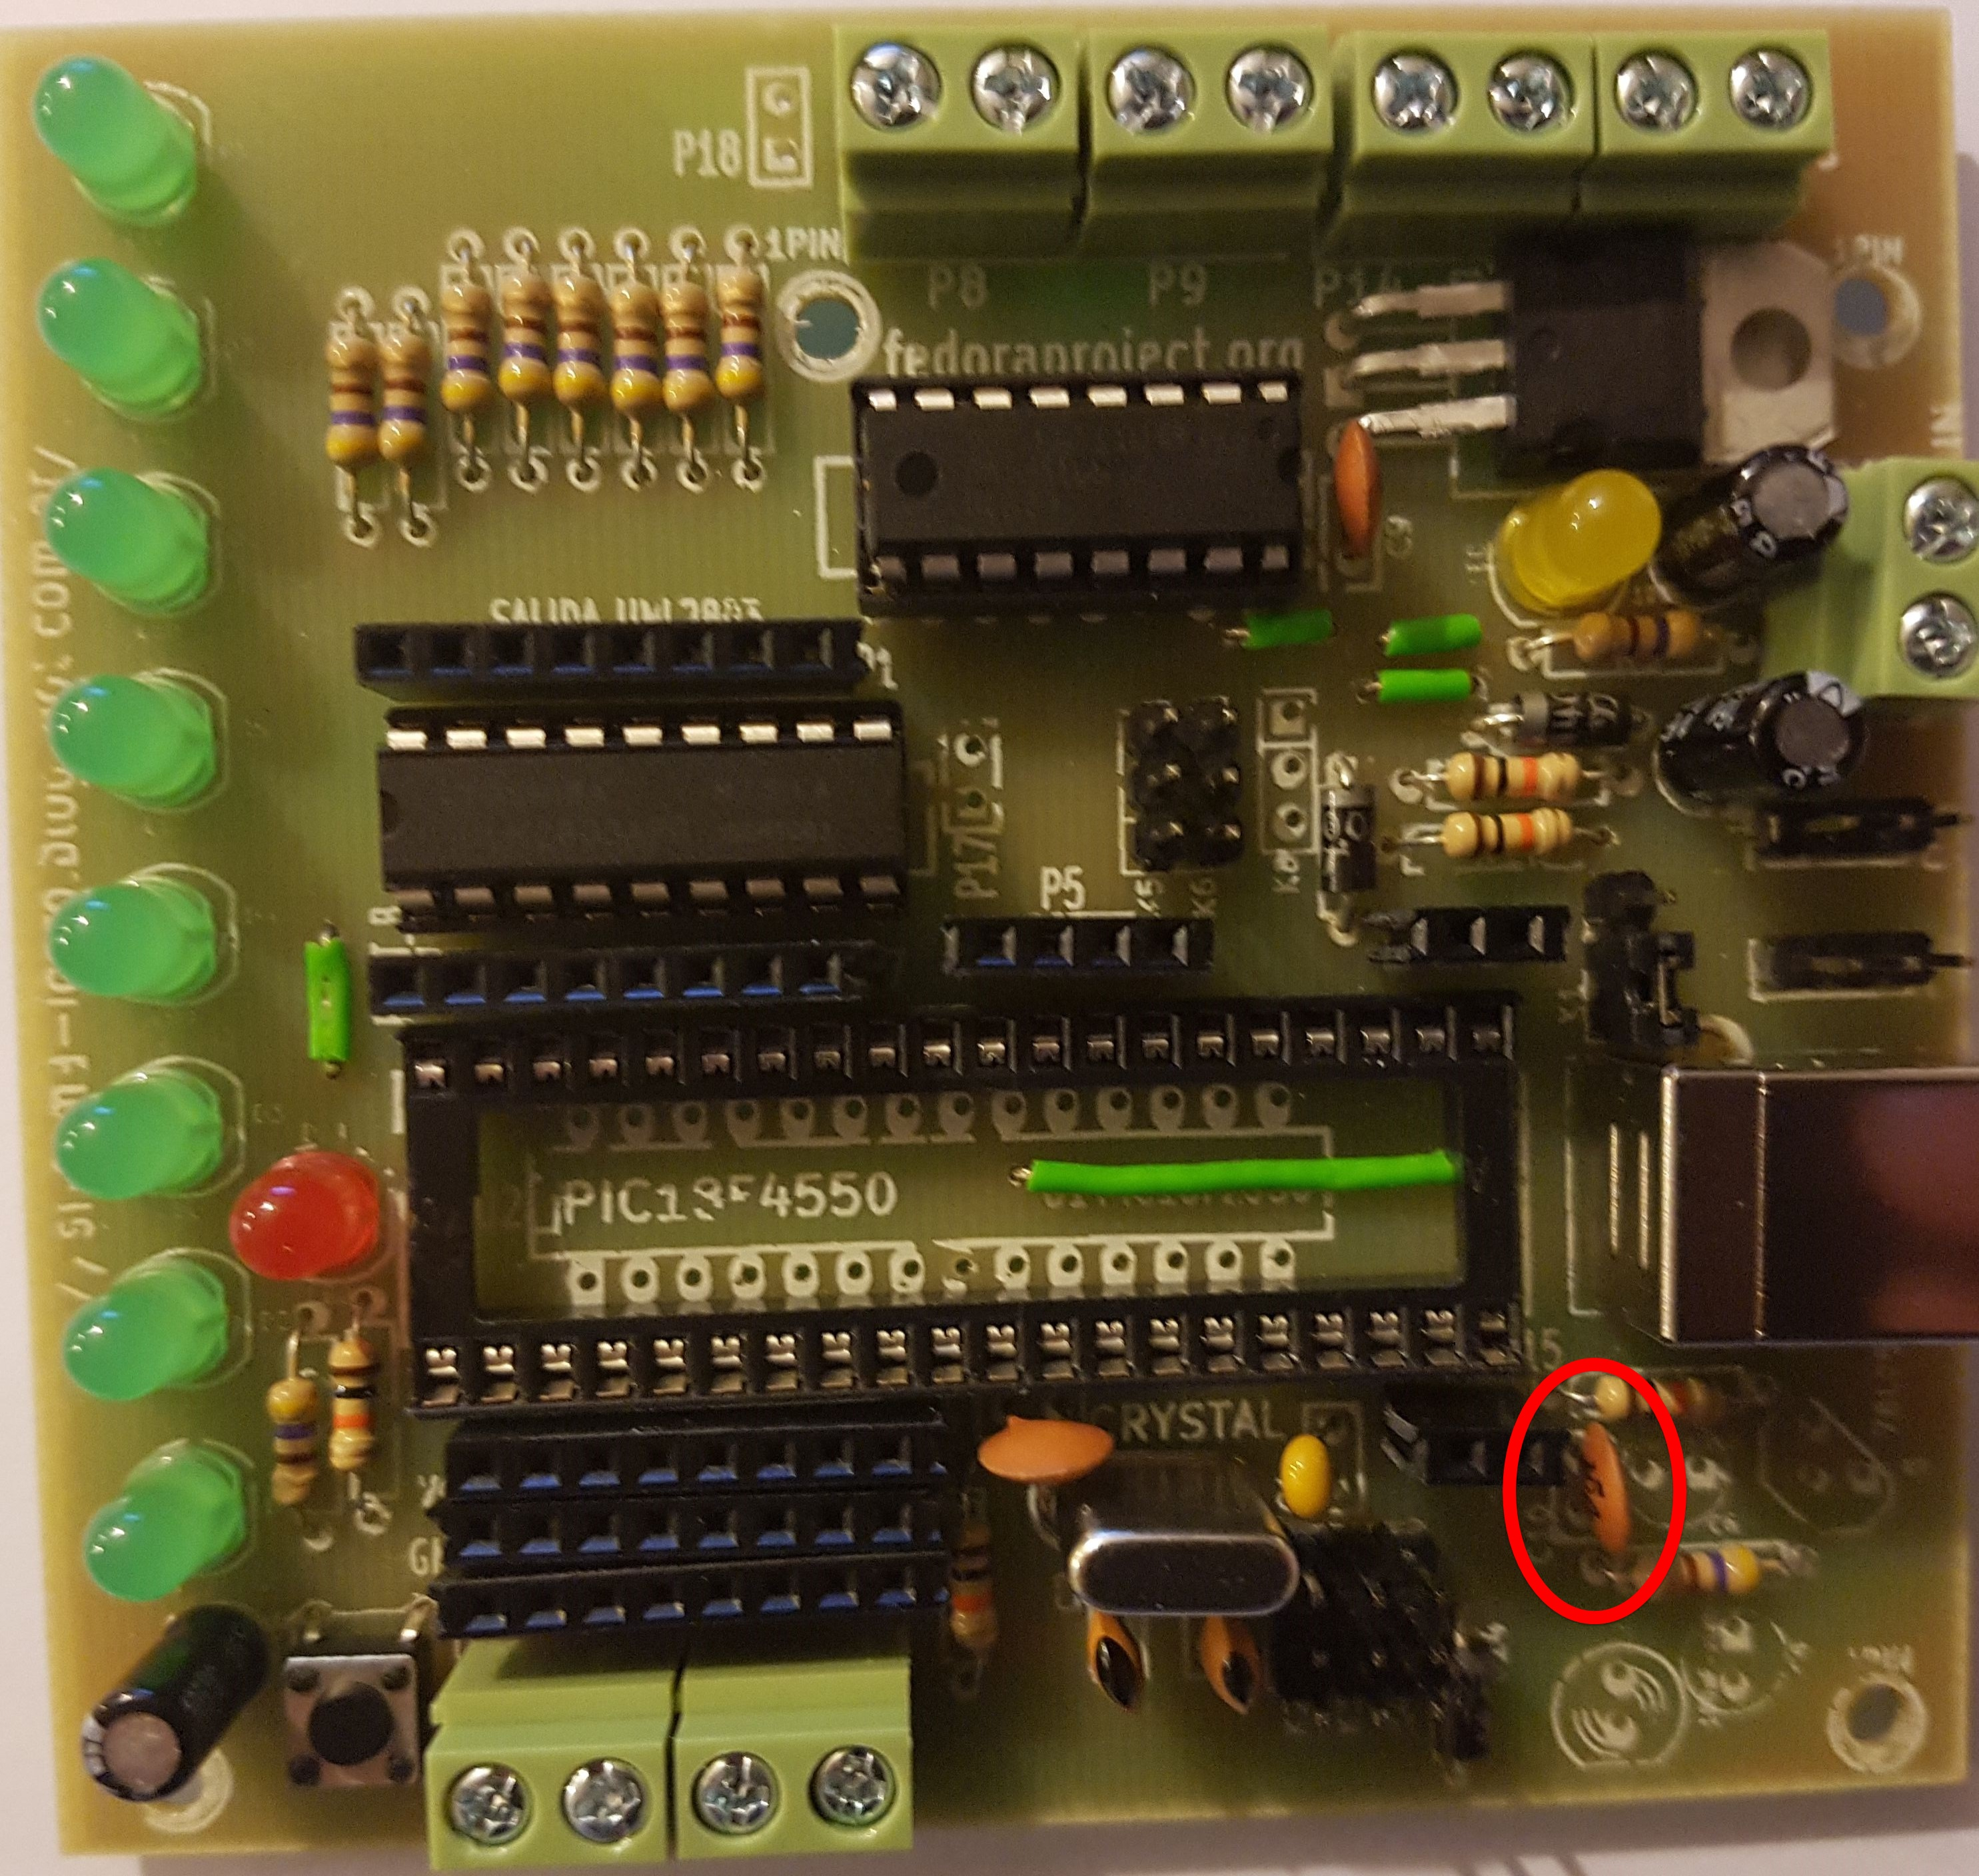
\includegraphics[width=0.8\linewidth]{Modulo_6/M6_6}
	\caption{Módulo 6 - Paso 6}
	\label{fig:M6_6}
\end{figure}

\newpage

\section{Paso 7:}

Instalar capacitores electrolíticos 100uF C6 y C8

\begin{figure}[h]
	\centering
	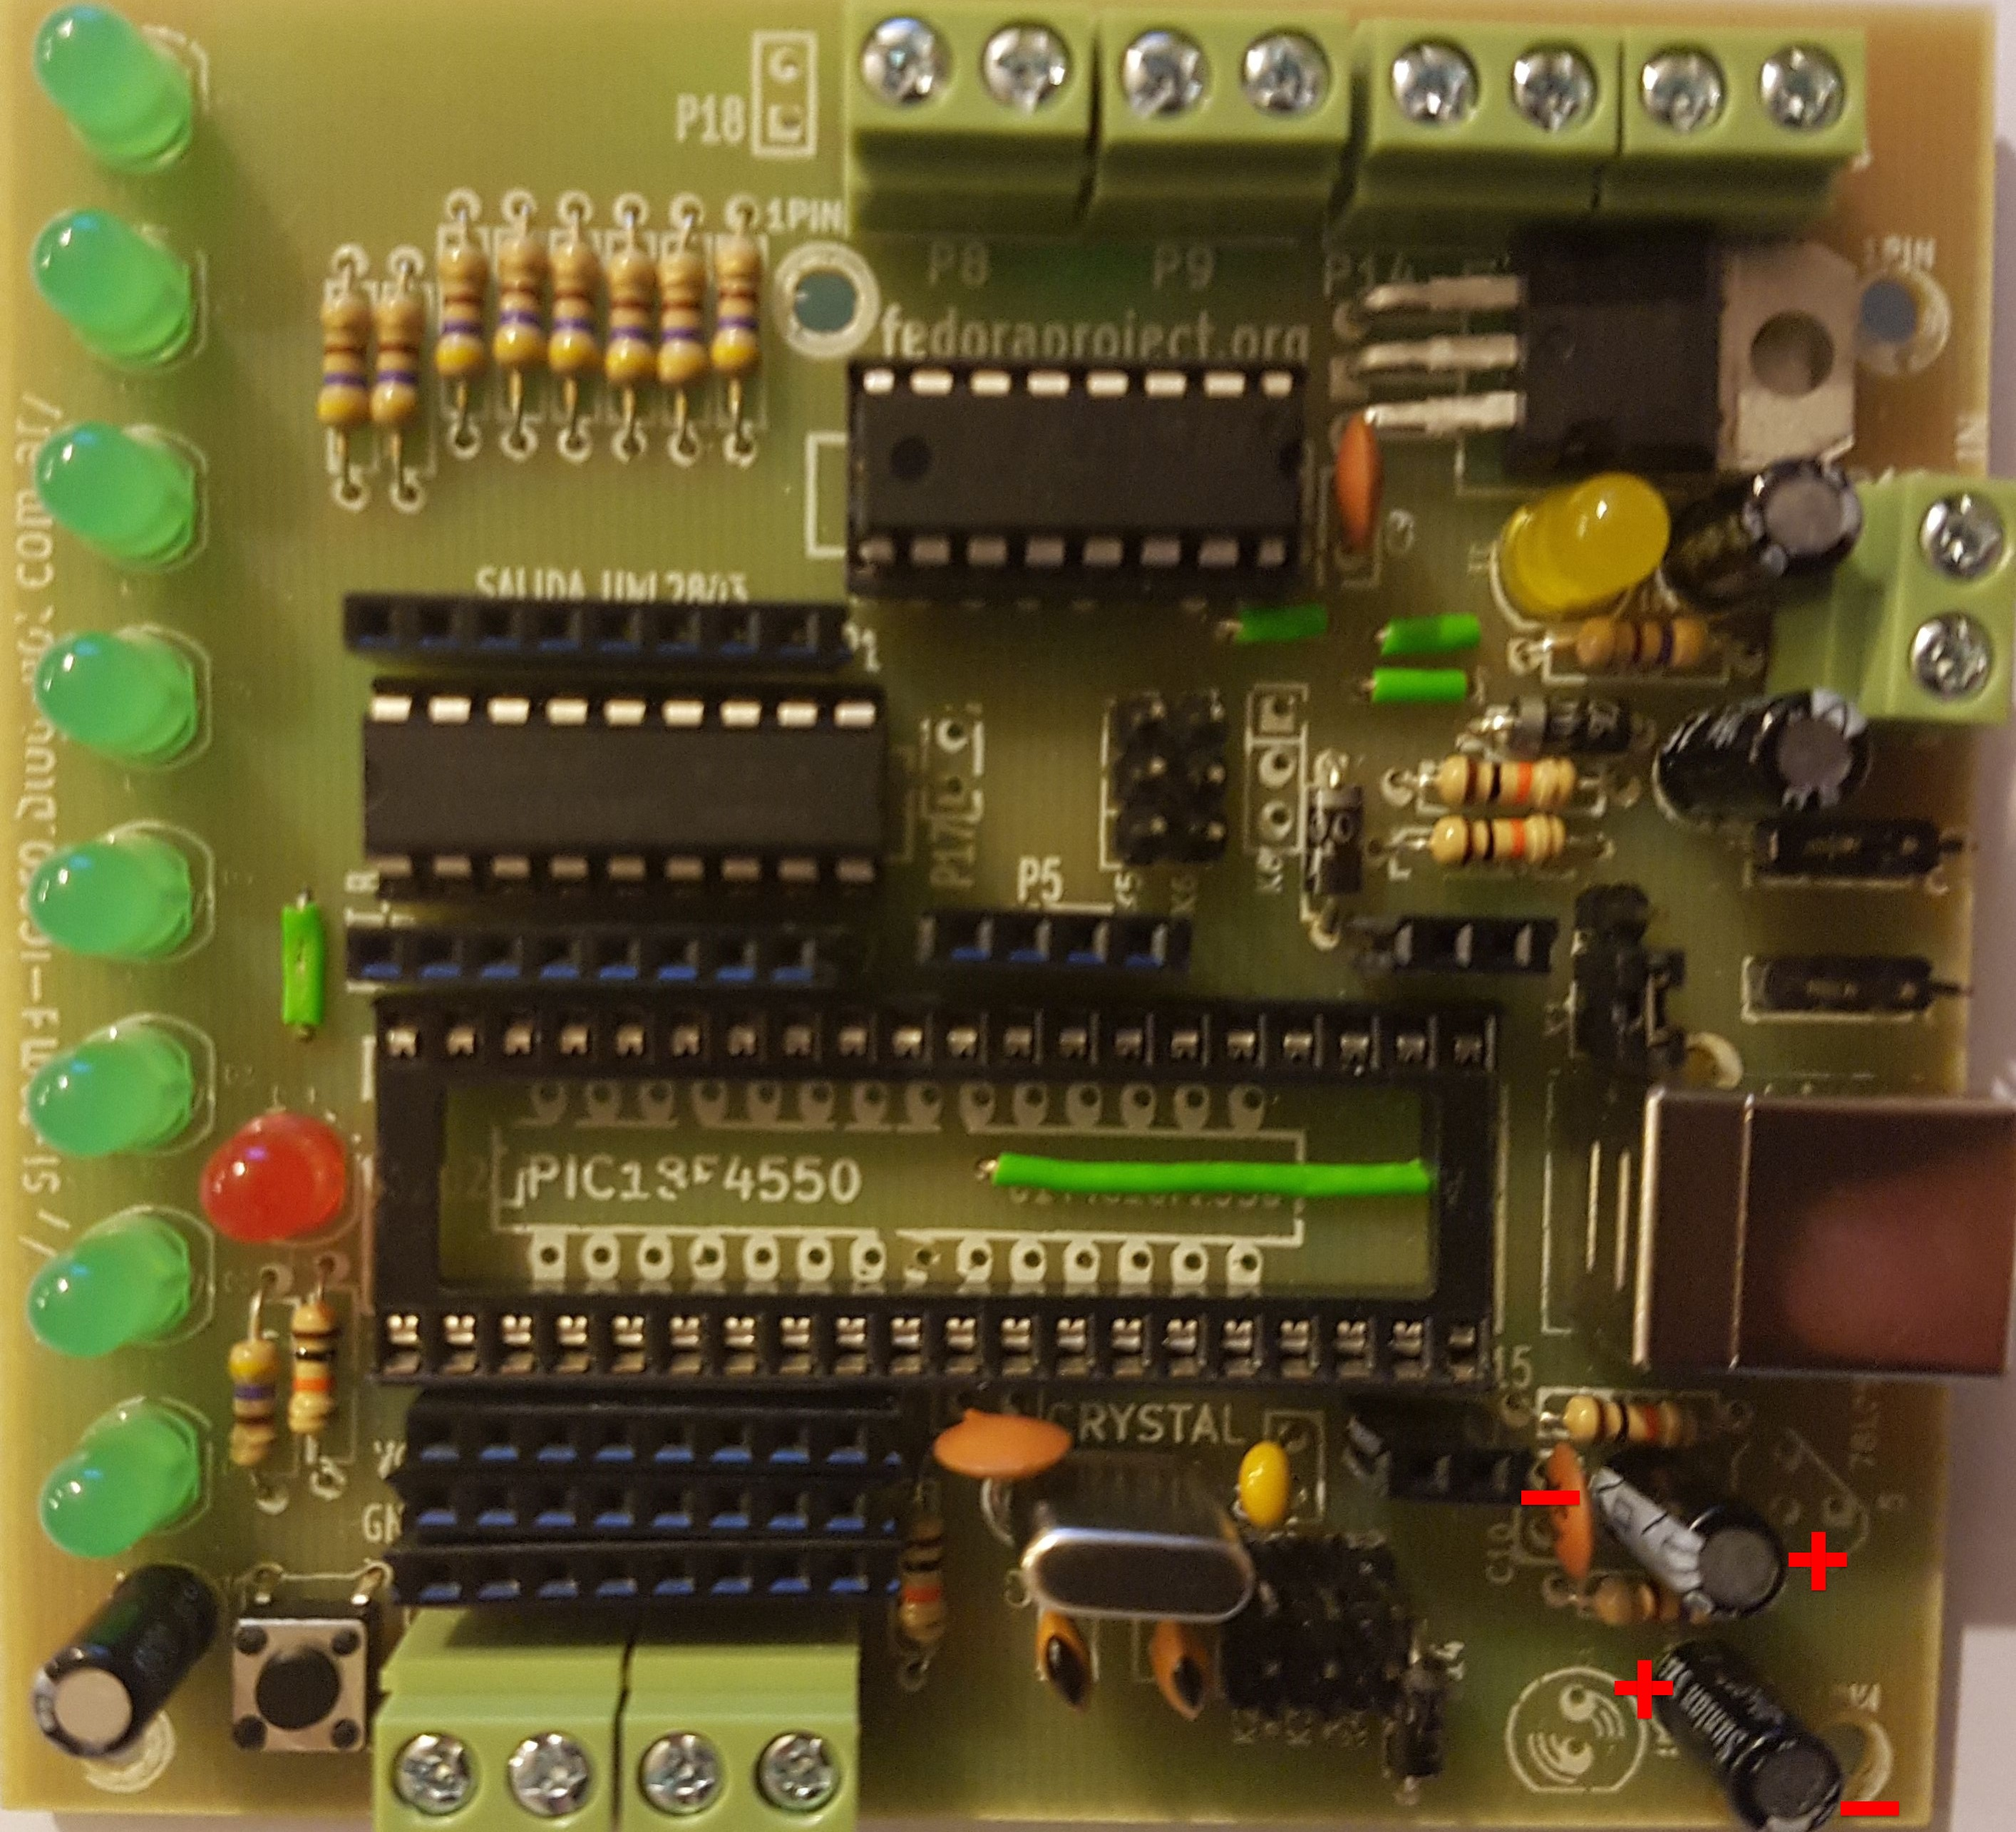
\includegraphics[width=0.8\linewidth]{Modulo_6/M6_7}
	\caption{Módulo 6 - Paso 7}
	\label{fig:M6_7}
\end{figure}

\newpage

\section{Paso 8:}

Instalar regulador 78L05. U5. Se recomienda doblar la pata del centro hacia atrás en 45 grados y luego hacerle otro doblez para que quede paralela a las demás.


\begin{figure}[h]
	\centering
	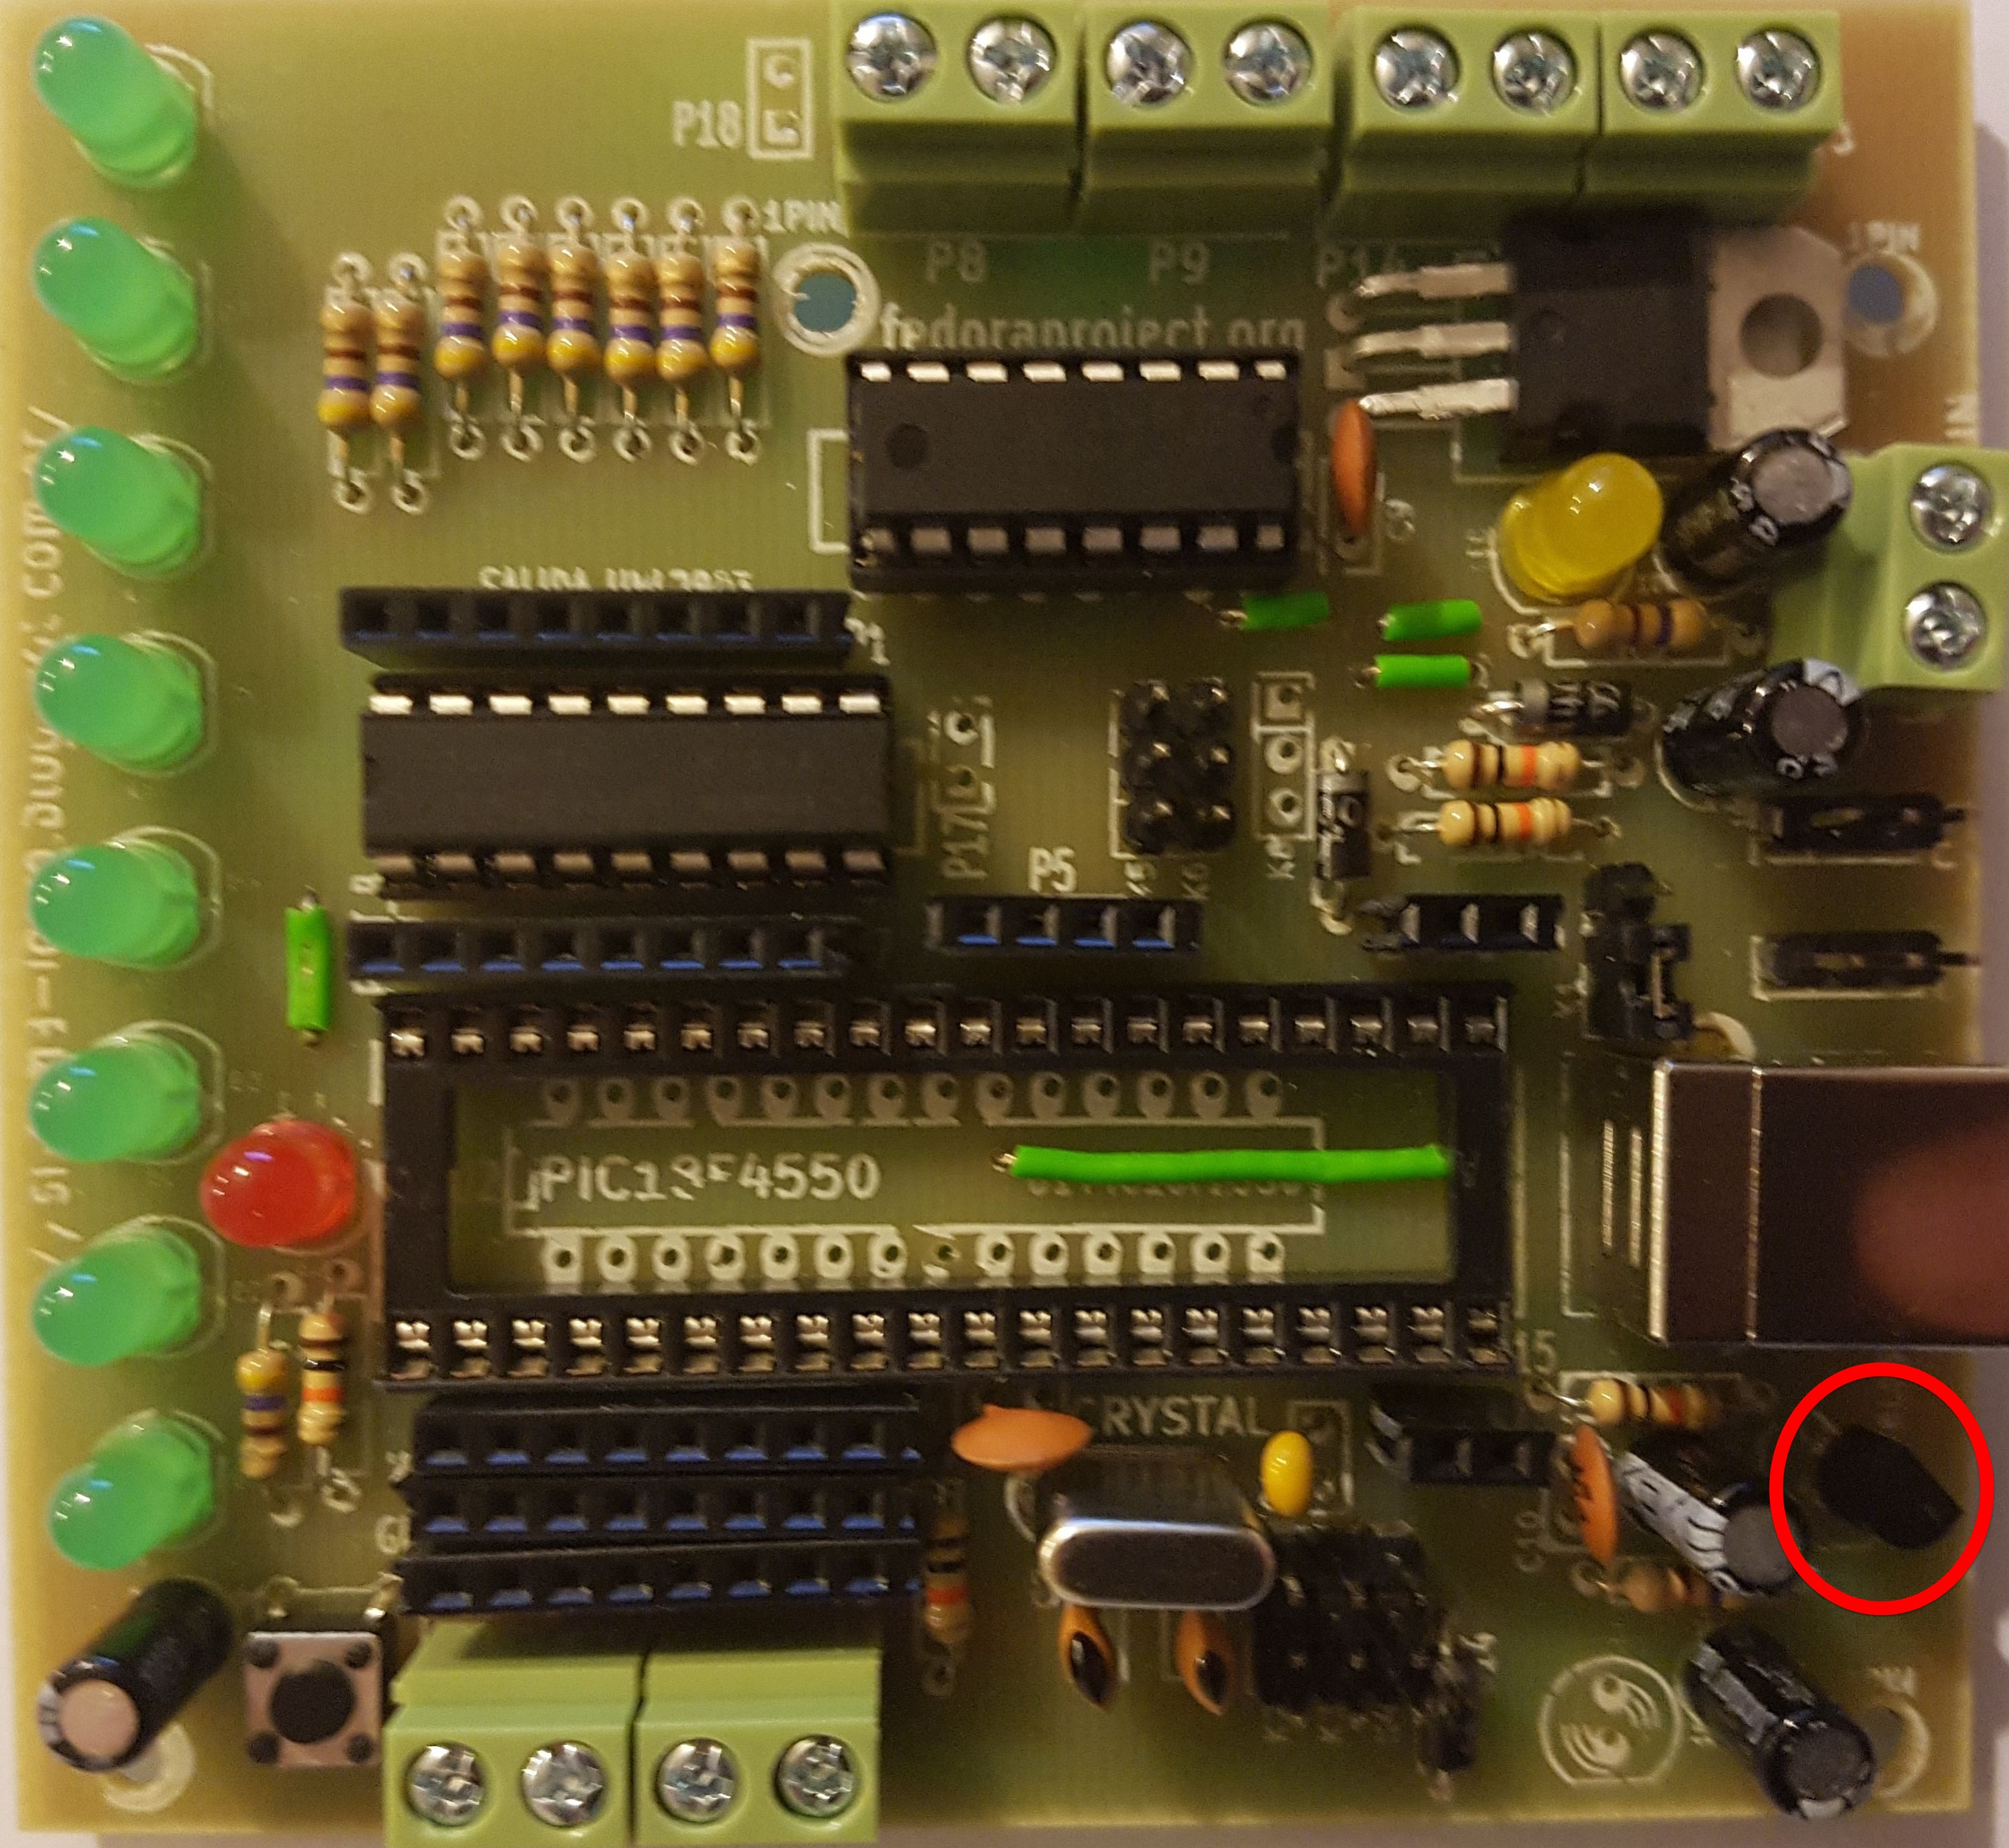
\includegraphics[width=0.8\linewidth]{Modulo_6/M6_8}
	\caption{Módulo 6 - Paso 8}
	\label{fig:M6_8}
\end{figure}

\newpage

\section{Paso 9:}

Instalar led de alimentación de la placa. D13 Se recomienda color verde.

\begin{figure}[h]
	\centering
	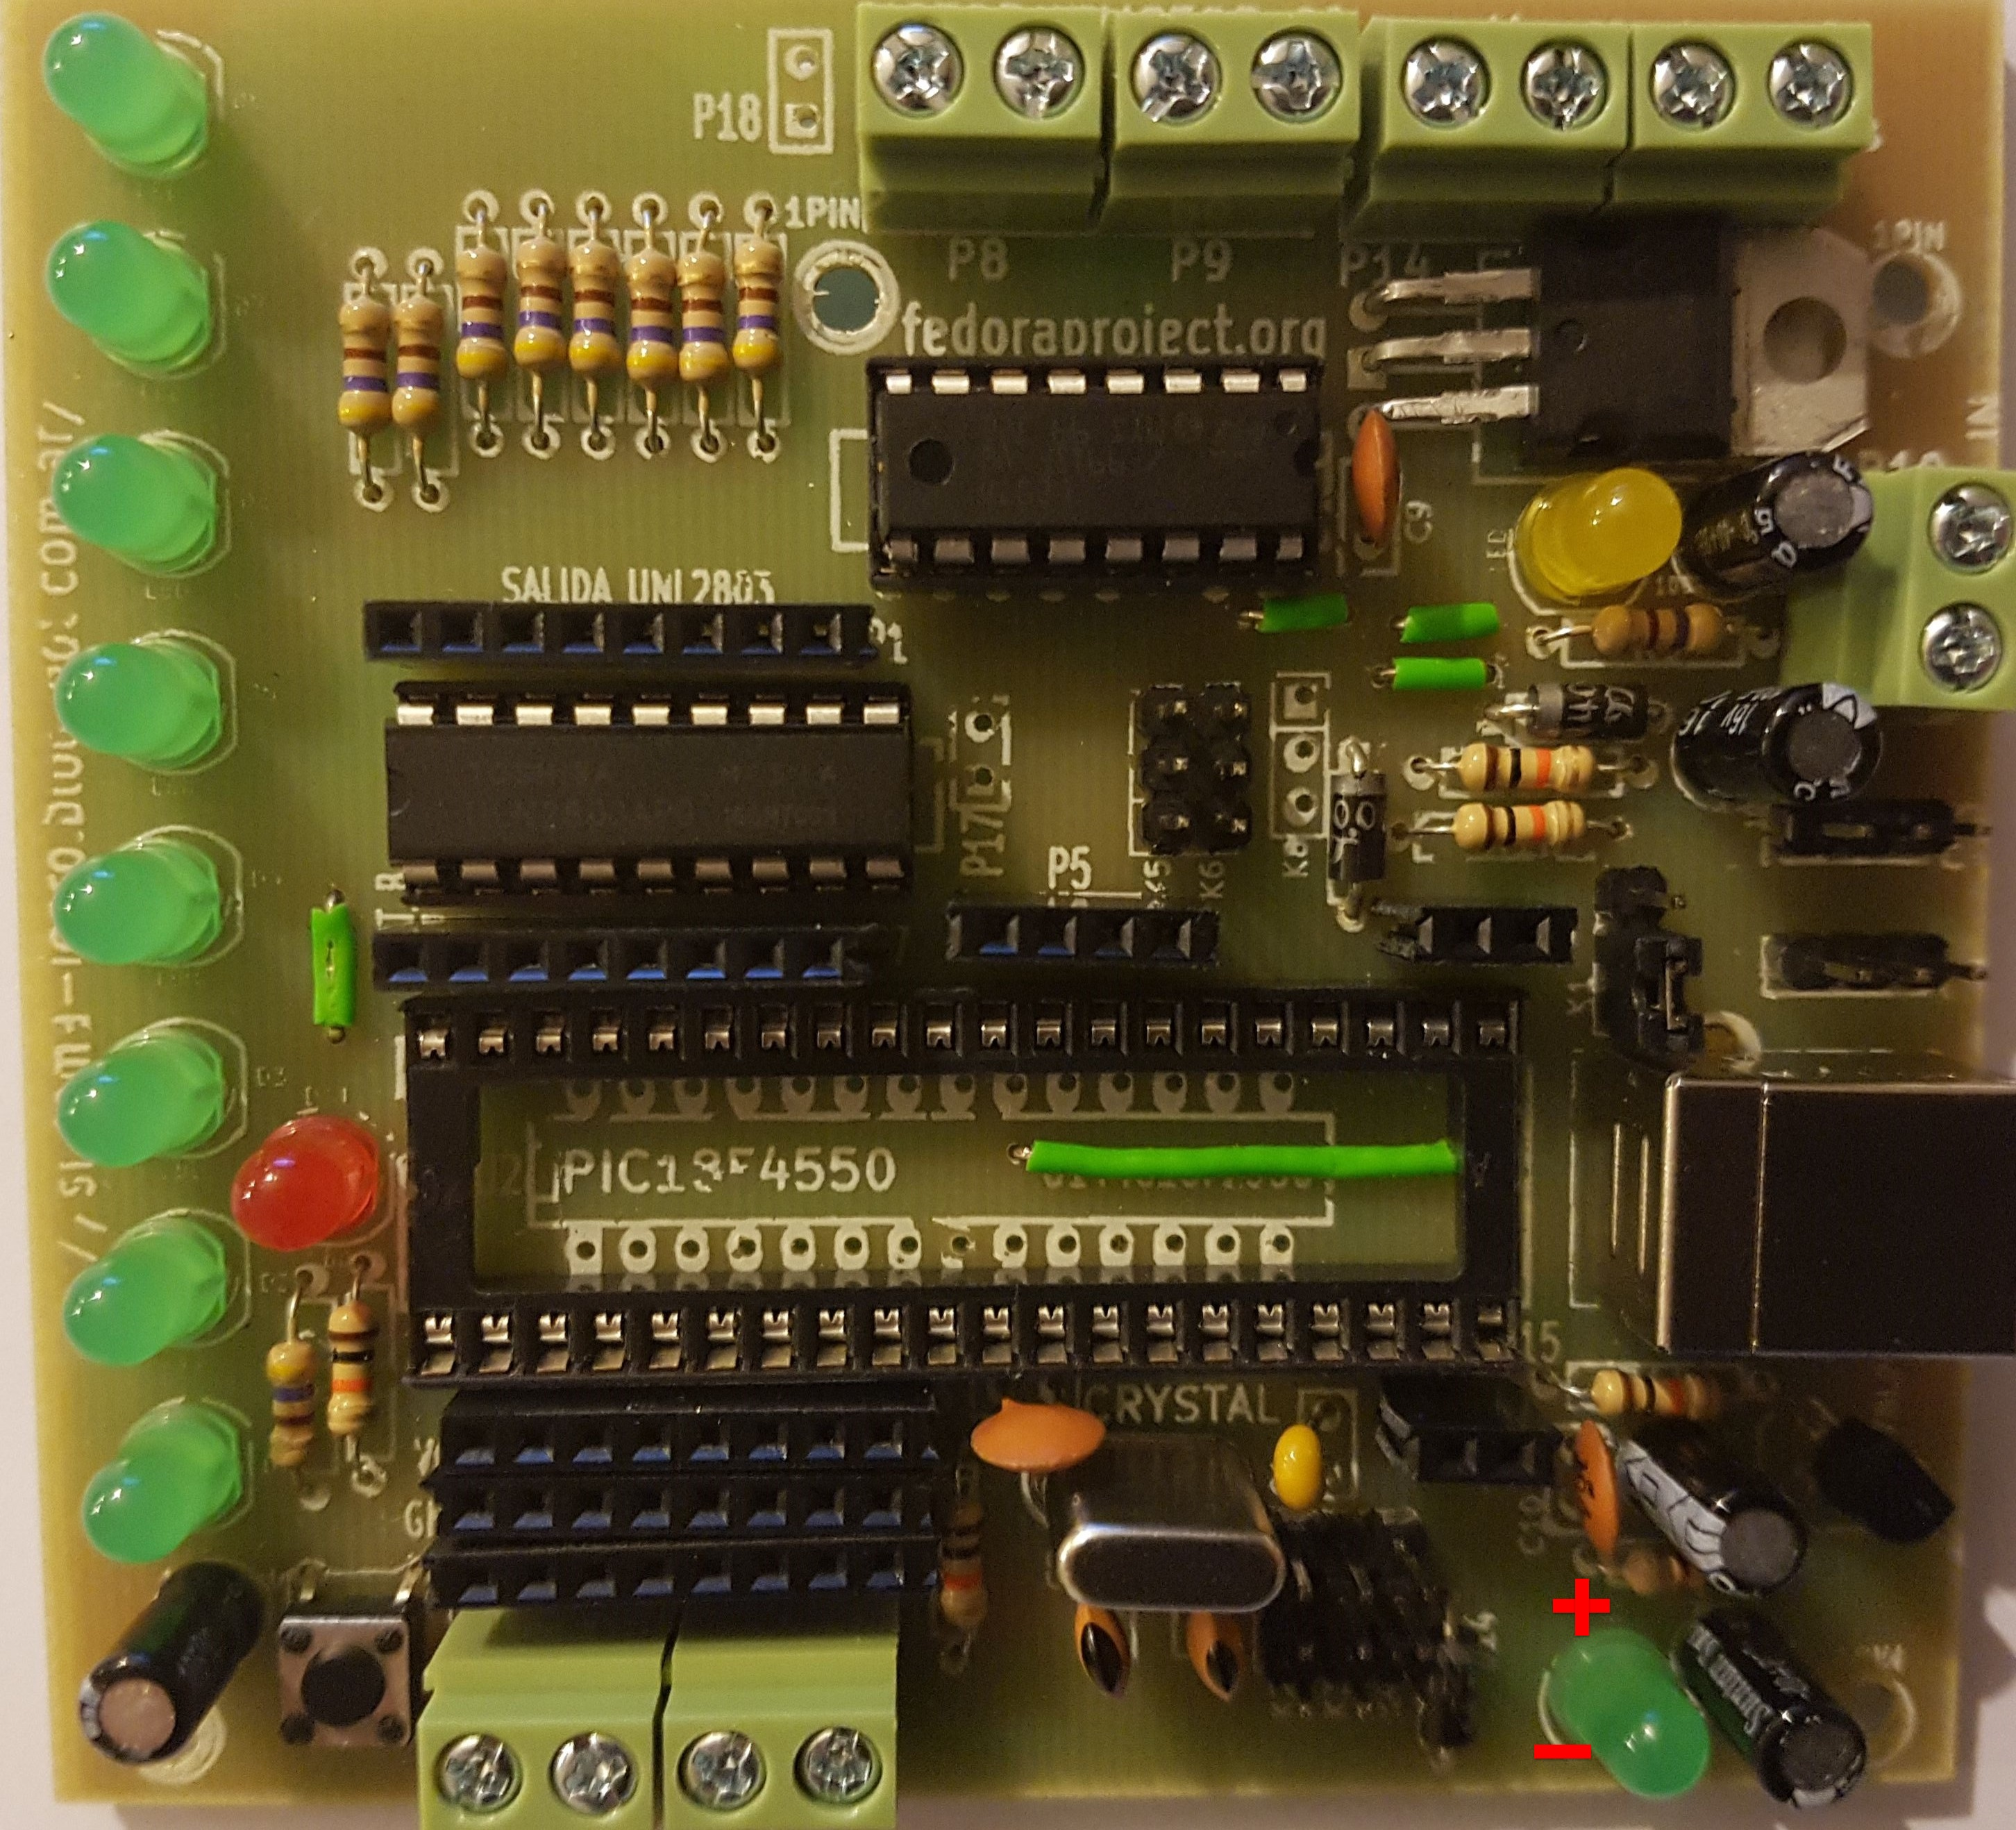
\includegraphics[width=0.8\linewidth]{Modulo_6/M6_9}
	\caption{Módulo 6 - Paso 9}
	\label{fig:M6_9}
\end{figure}

\newpage

\section{Paso 10:}

Instalar tira de pines machos en el selector de voltaje. K8

\begin{figure}[h]
	\centering
	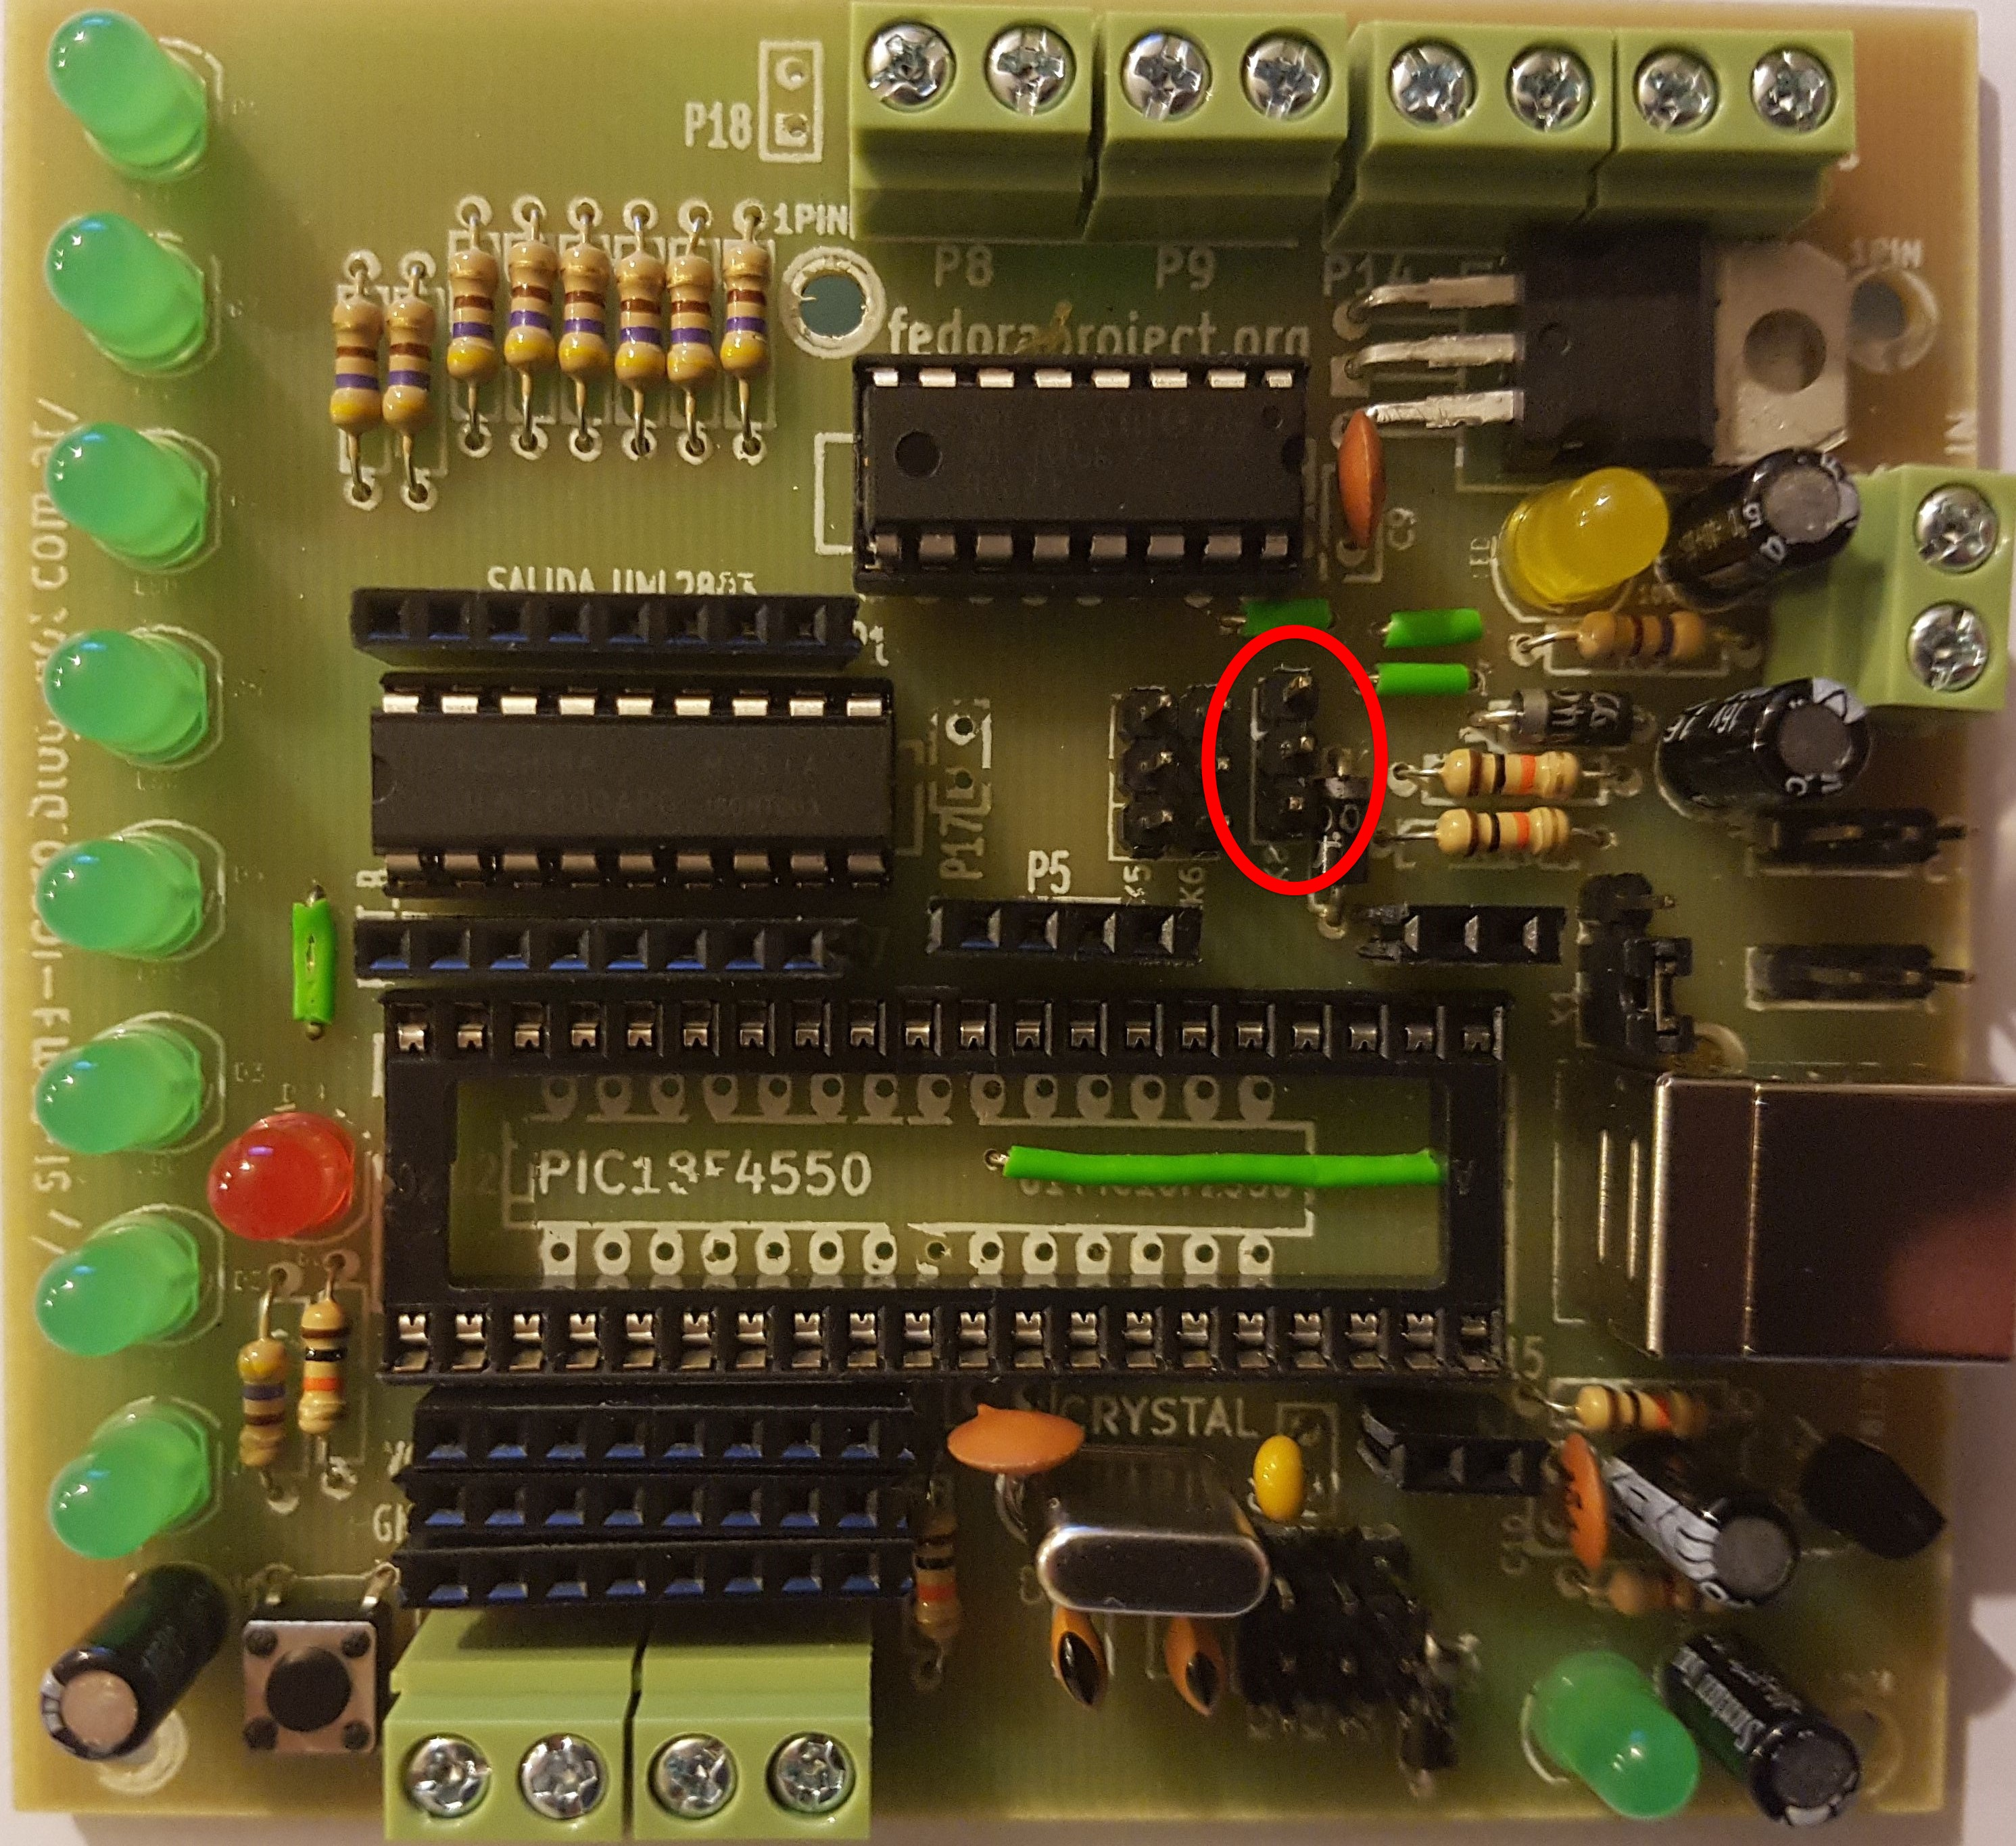
\includegraphics[width=0.8\linewidth]{Modulo_6/M6_10}
	\caption{Módulo 6 - Paso 10}
	\label{fig:M6_10}
\end{figure}

\newpage

\section{Paso 11:}

Instalar jumper en K8 del lado del micro

\begin{figure}[h]
	\centering
	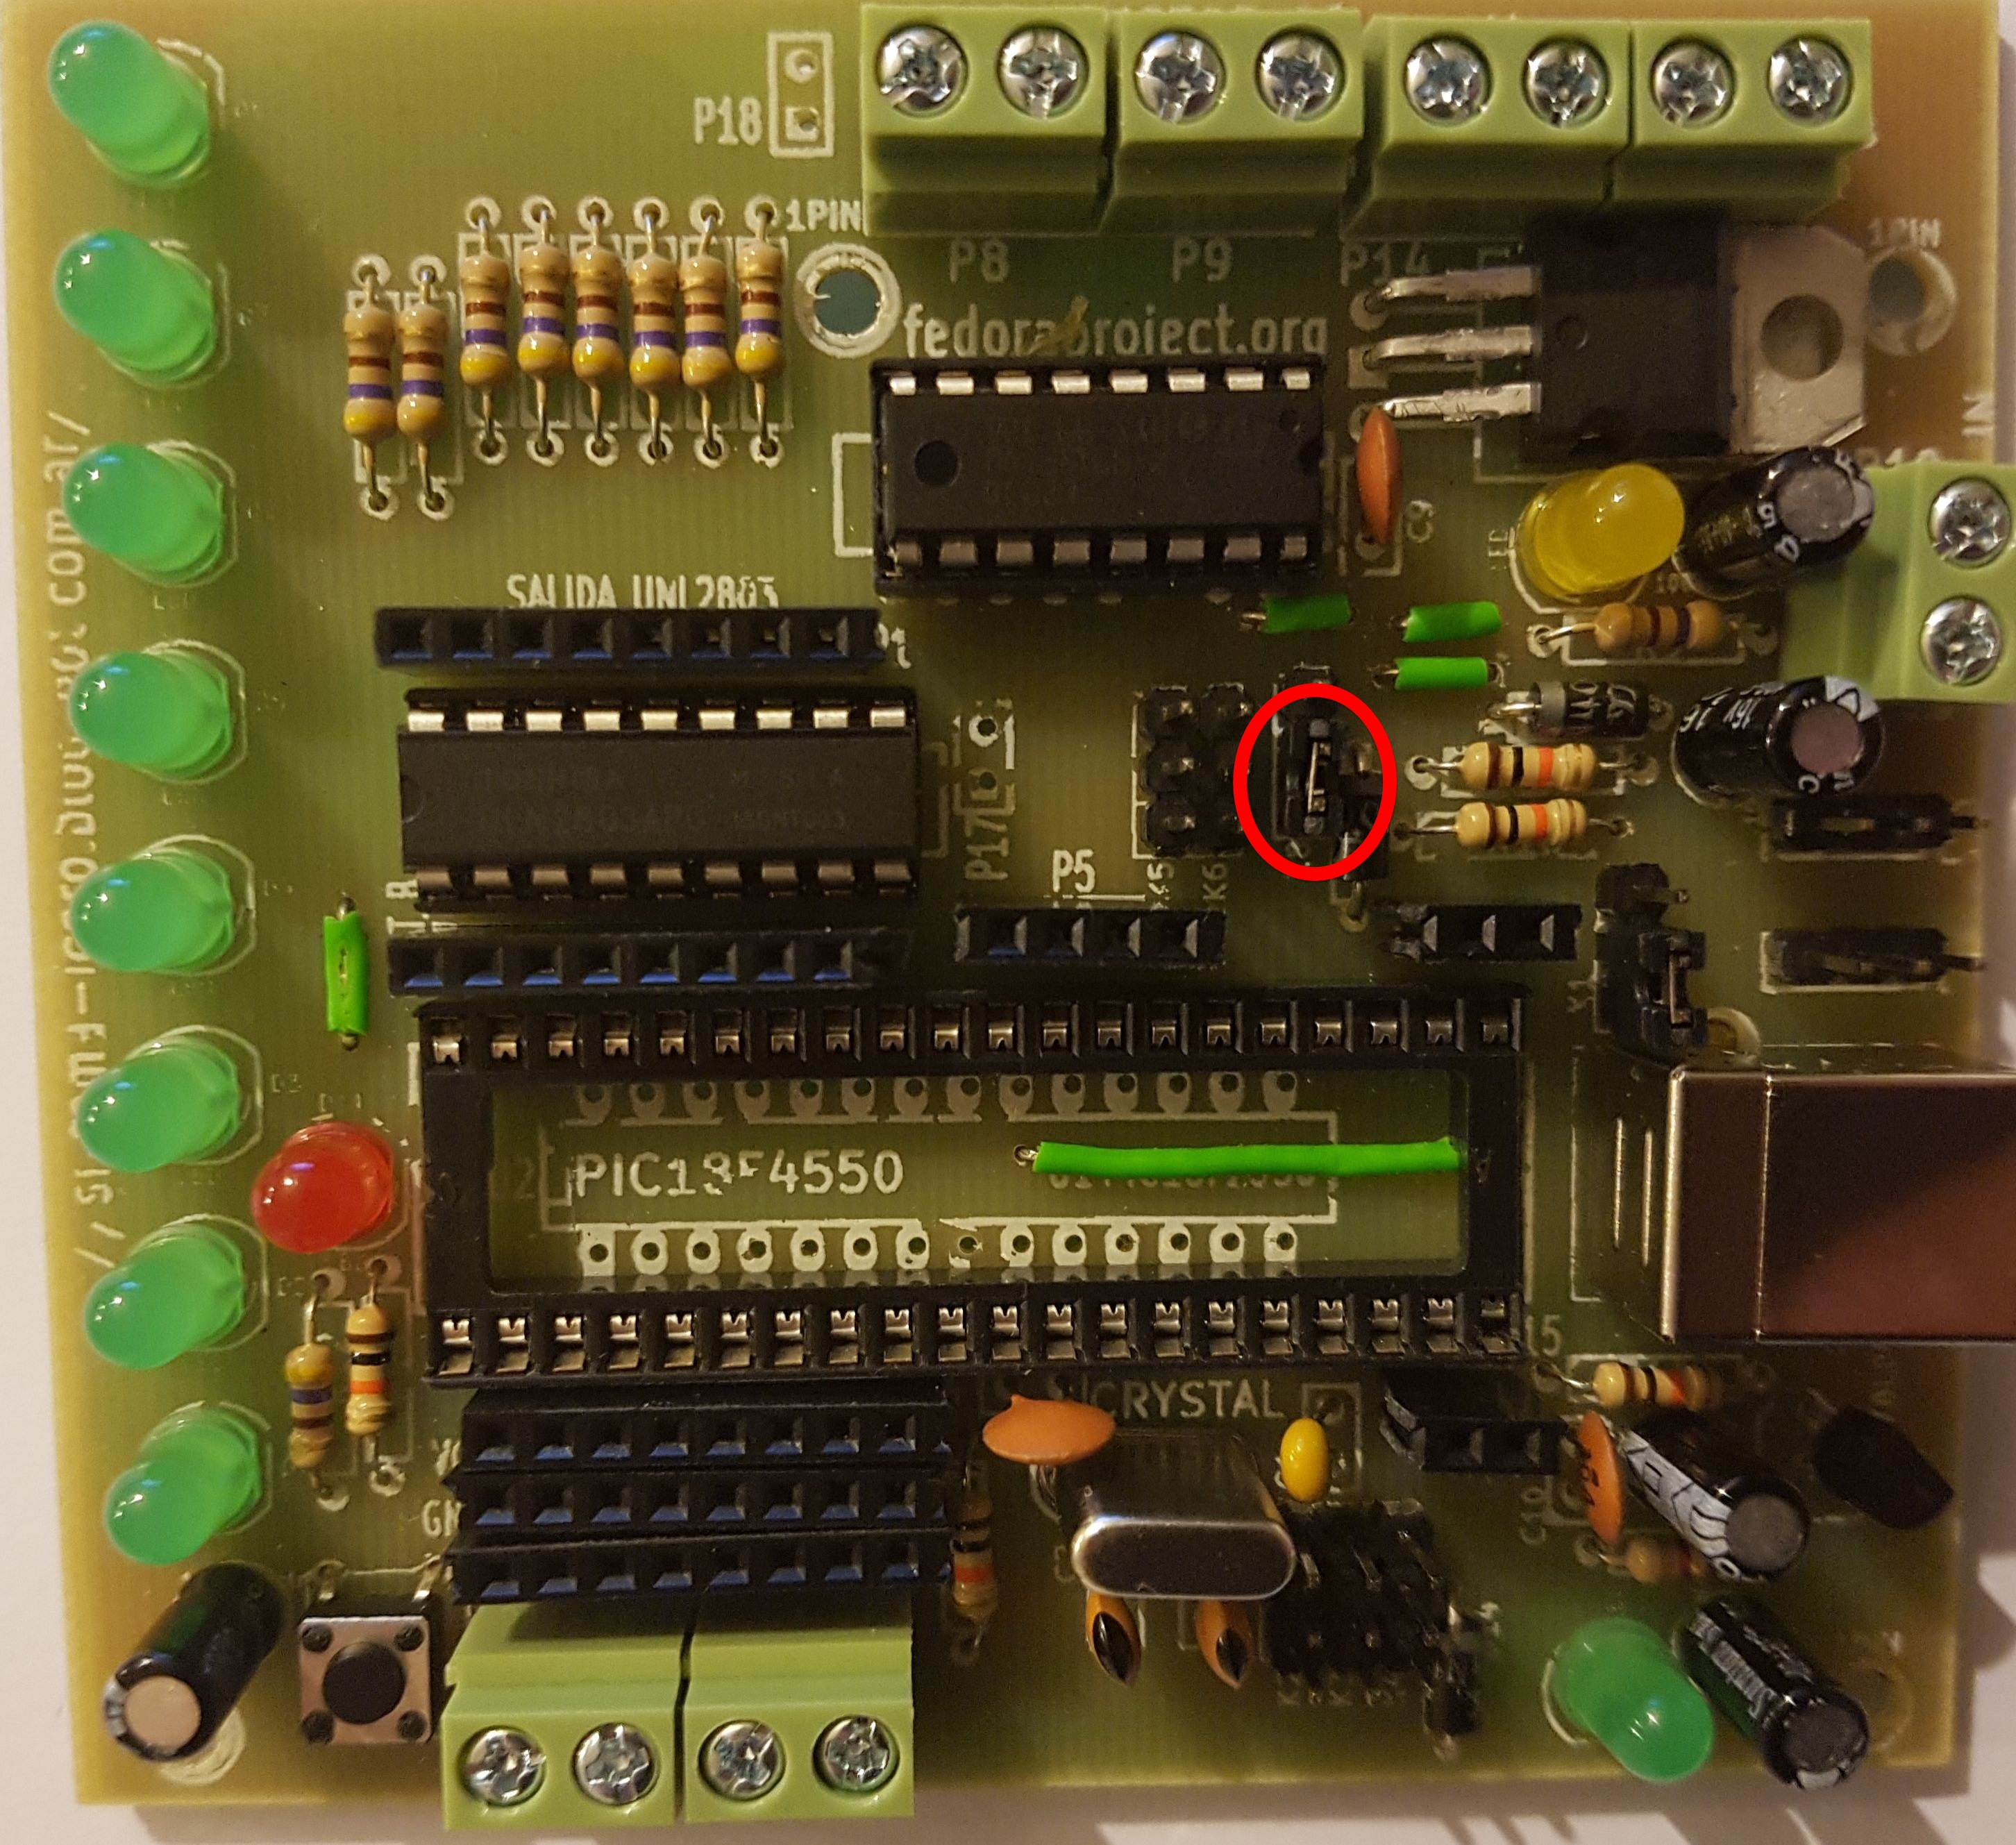
\includegraphics[width=0.8\linewidth]{Modulo_6/M6_11}
	\caption{Módulo 6 - Paso 11}
	\label{fig:M6_11}
\end{figure}

\newpage

\section{Paso 12:}

Instalar tira de pines hembras P17 (es una toma de corriente)

\begin{figure}[h]
	\centering
	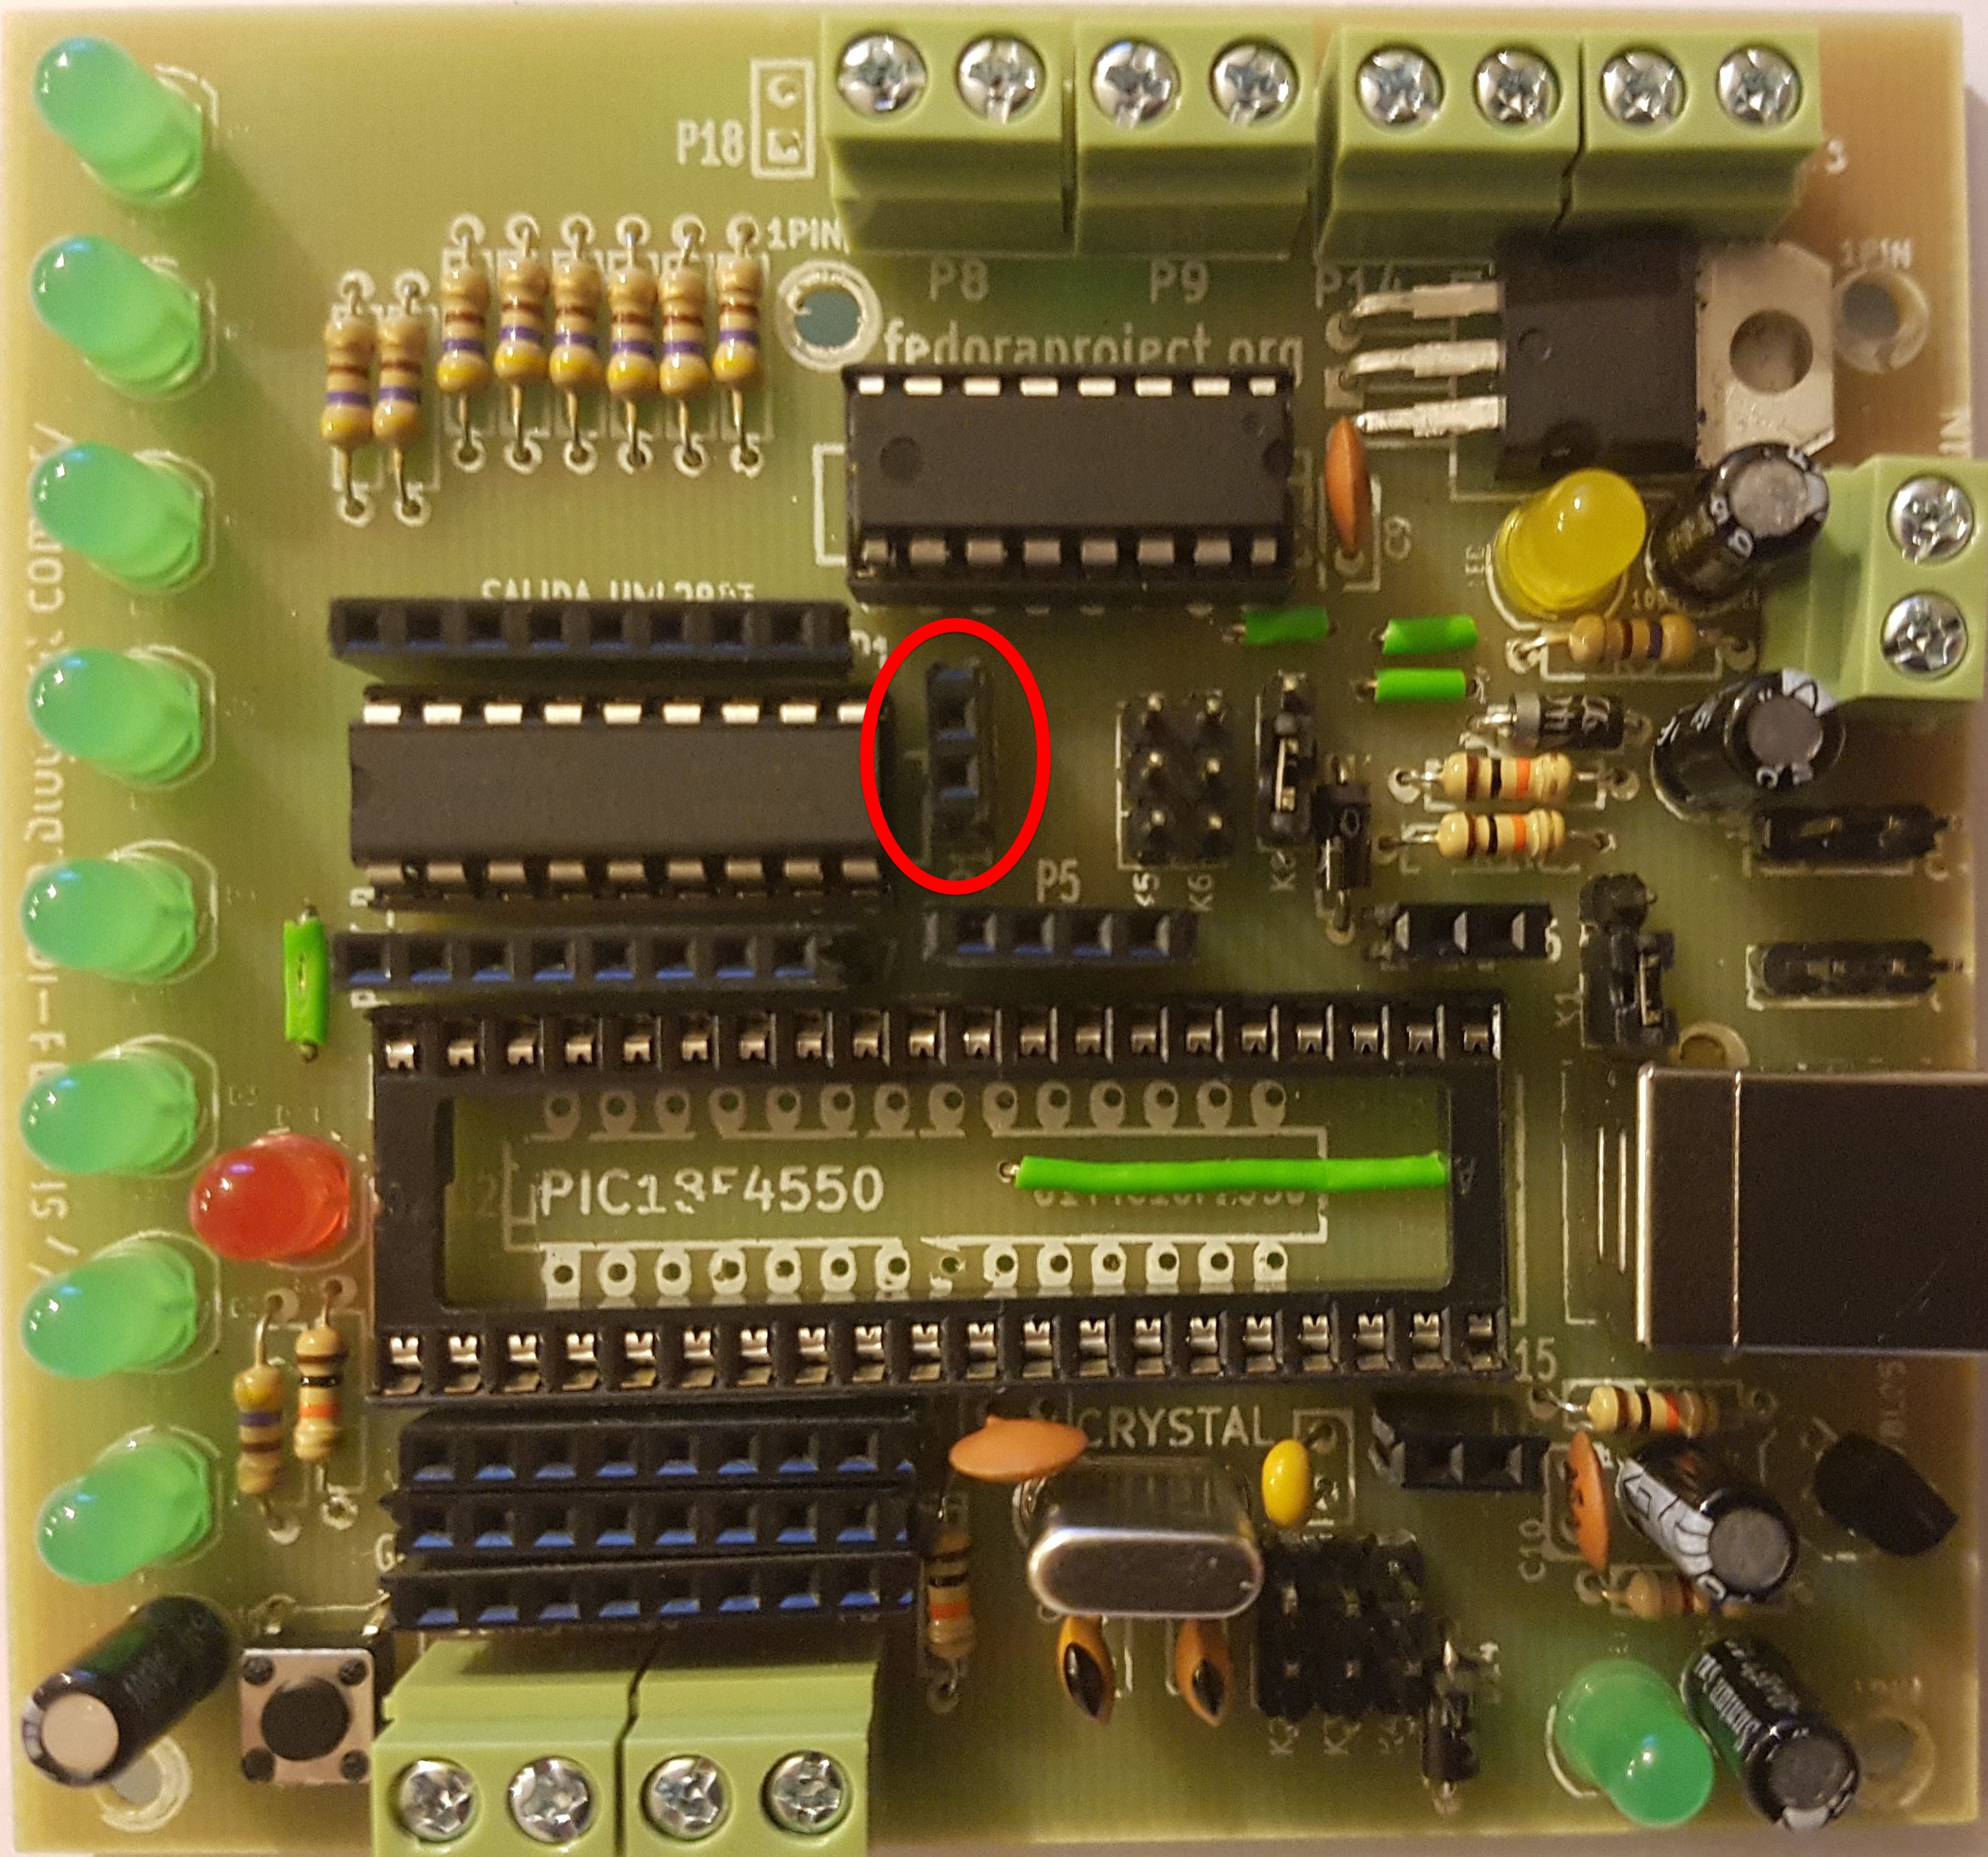
\includegraphics[width=0.8\linewidth]{Modulo_6/M6_12}
	\caption{Módulo 6 - Paso 12}
	\label{fig:M6_12}
\end{figure}

\newpage

\section{Paso 13:}

Instalar tira de pines hembras P18 (sirve para saltar un dio de protección y asegurar tener 5VDC. Solo ocupar en casos extremos y estando seguro del porque lo hace.

\begin{figure}[h]
	\centering
	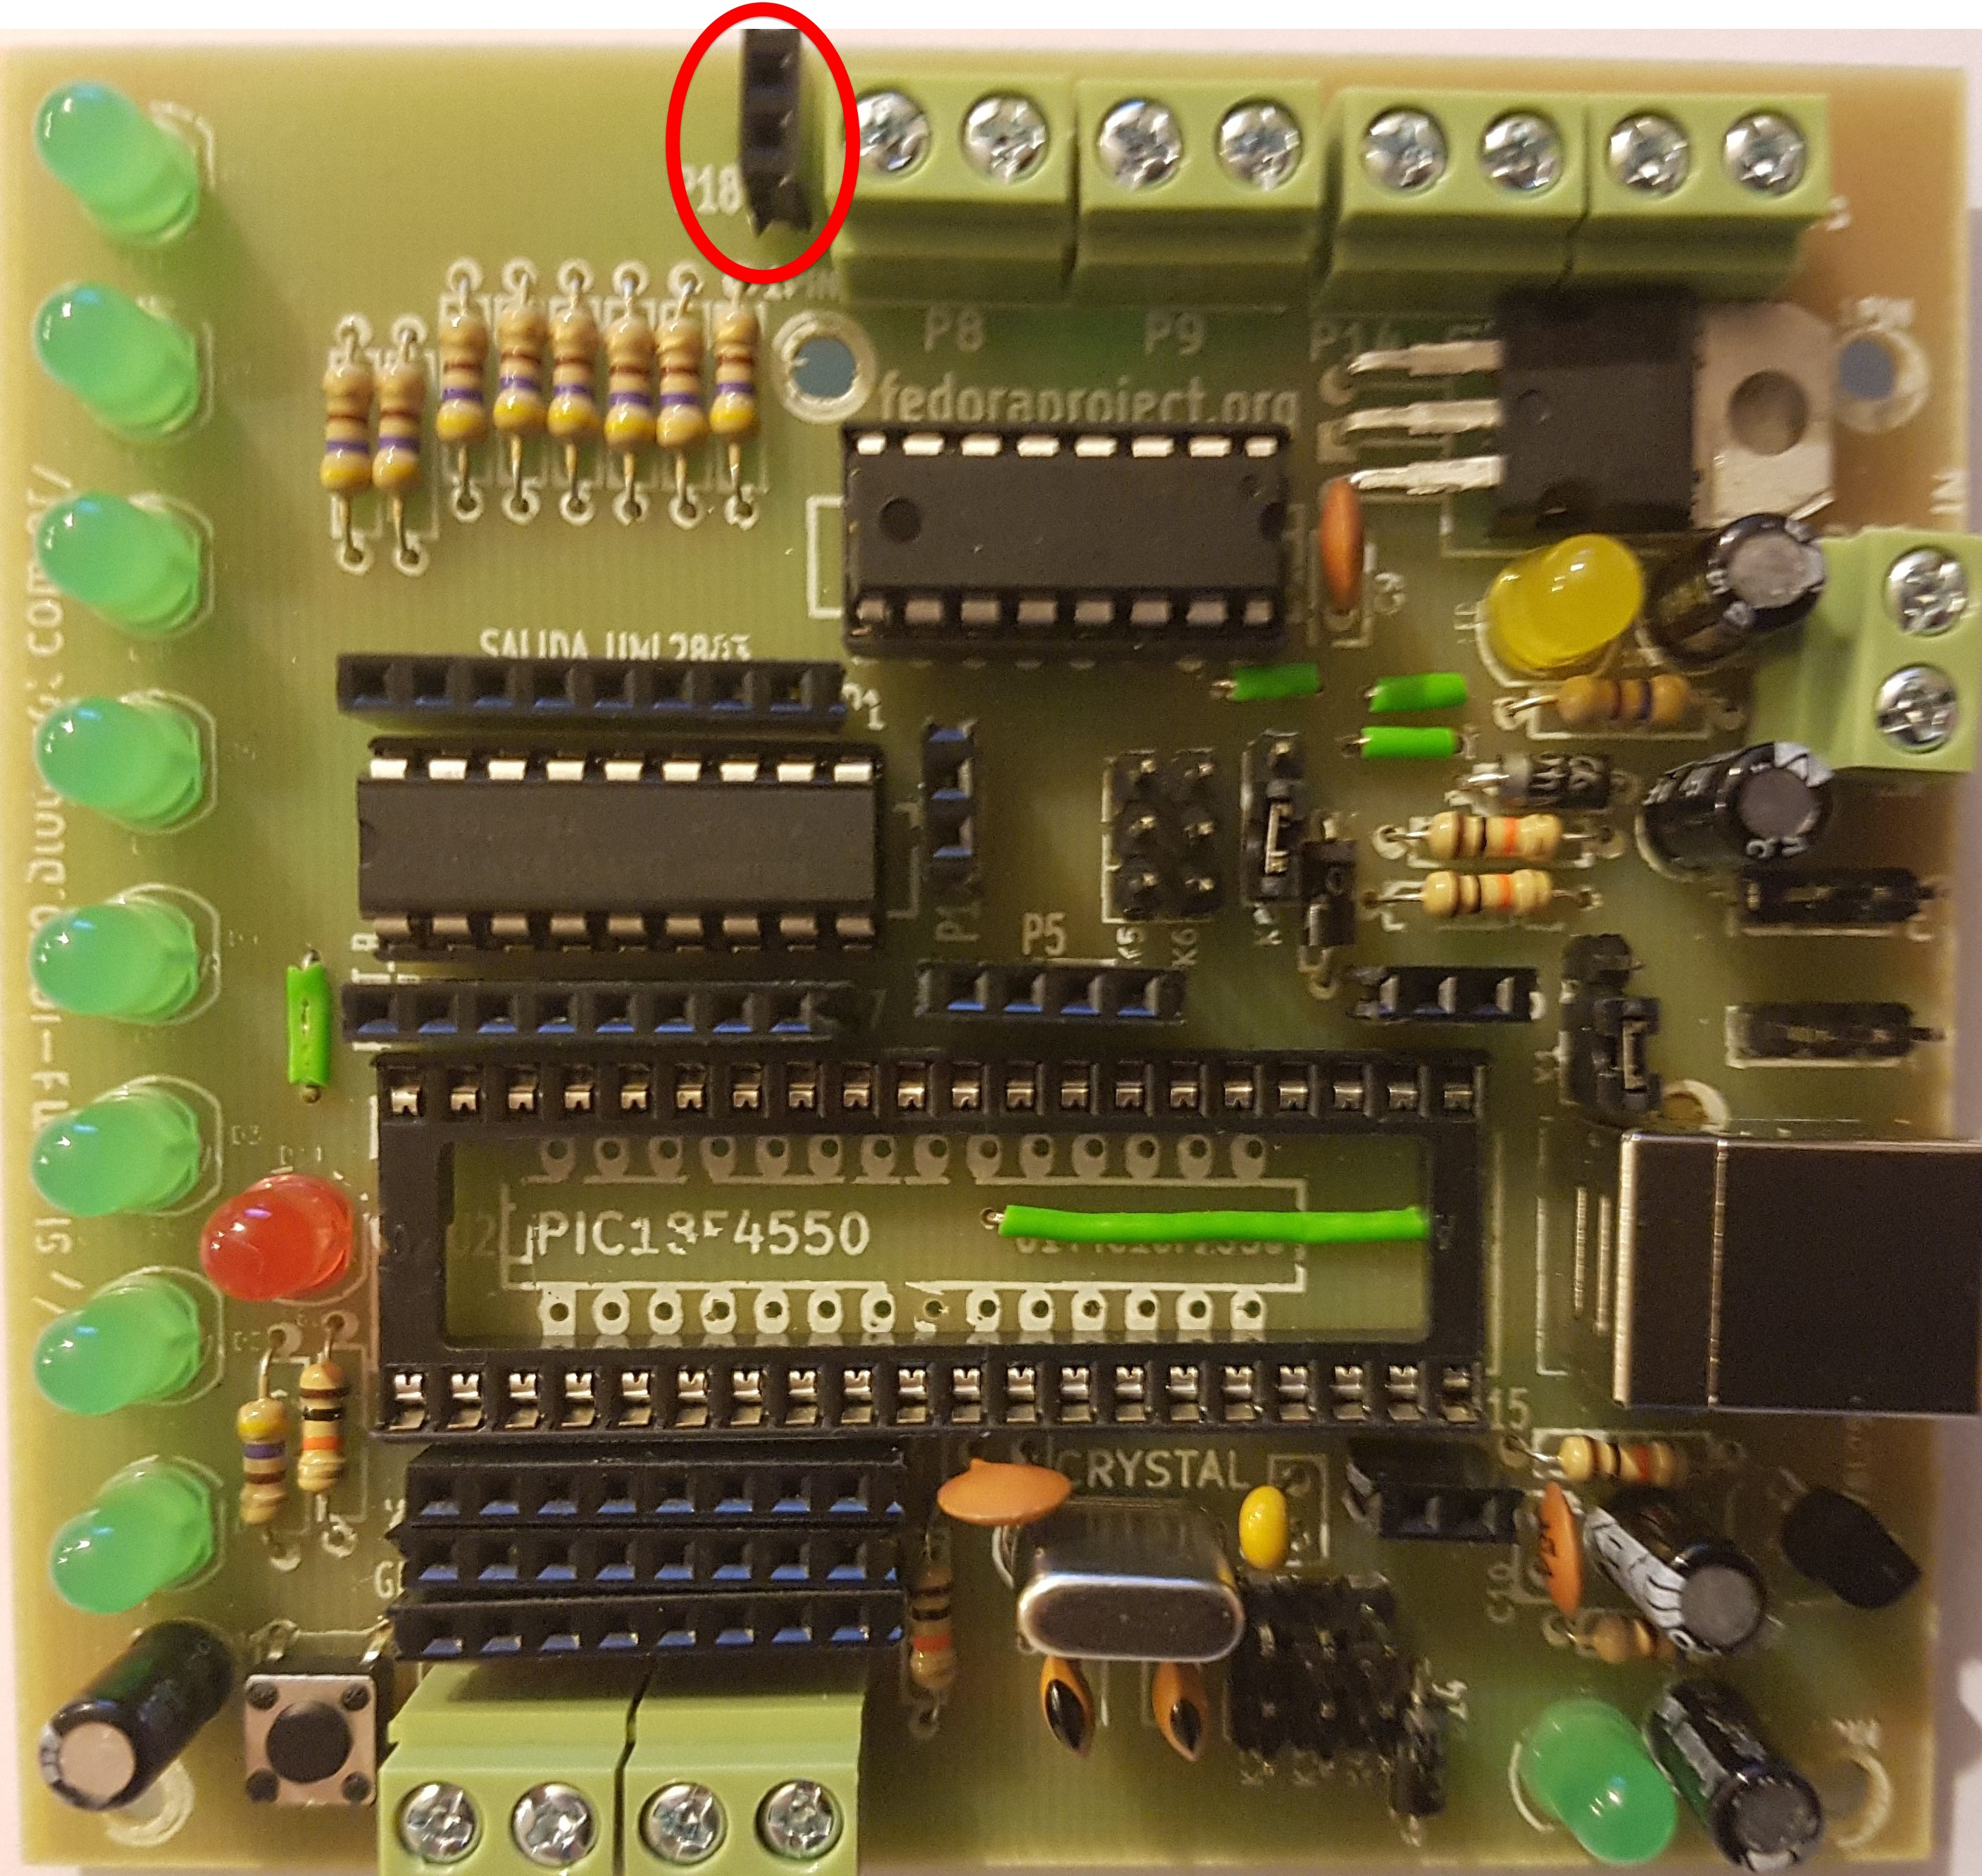
\includegraphics[width=0.8\linewidth]{Modulo_6/M6_13}
	\caption{Módulo 6 - Paso 13}
	\label{fig:M6_13}
\end{figure}